\chapter{Machine Learning and Neural Networks}\label{ch:neural-networks}
In this chapter, we provide an overview of Machine Learning and neural networks. We start with a short introduction to Machine Learning, laying out the foundations on how learning from data is possible, as well as more practical aspects about the selection and evaluation of machine learning models. In Section \ref{sec:nn}, we briefly review the core concepts about \glspl{nn}, such as the procedure by which they are trained, the loss functions they optimize, and how they are regularized.

\section{Machine Learning}\label{sec:ml}
Many real-world phenomena are not clearly understood, or cannot be characterized in terms of simple mathematical equations. However, one can usually collect quantitative and/or qualitative measurements about them, and observe their effects in the environment where they manifest. \gls{ml} is a branch of Artificial Intelligence that studies algorithms and provides tools to \emph{learn} these unknown processes from data. According to Mitchell, \keyword{learning} is defined as improving at some task from experience \citep{mitchell1997ml}. To start off, let us first briefly describe the key components of a learning system in detail, introducing other useful notation, definitions and concepts along the way:

\begin{itemize}
    \item the \keyword{experience}, in the context of \gls{ml}, refers to
    the data which is available to the learner. Data is provided in the form
    of \emph{examples}, (also called \emph{observations} or \emph{data points}). Each example is a set of qualitative or quantitative measurements about some phenomenon of interest;
    \item the \keyword{task} refers to some function $\Target$ (called \emph{target function}) that the learner needs to estimate from data. \gls{ml} tasks are multiple, and of potentially very different nature. Three well-known examples of tasks are are \emph{classification}, where $\Target$ is a function that assigns a categorical \emph{label} to a data point; \emph{regression}, where $\Target$ associates a desired numerical quantity to a given example; and \emph{density estimation}, where $\Target$ is the probability density (or mass, for the discrete case) function from which the examples are drawn from;
    \item the \keyword{performance} is a function which returns a quantitative measurement of how \quotes{well} the task is being learned. For example, in a classification task, one can measure improvement measuring the \emph{accuracy} of the learner, \ie the proportion of correctly classified examples out of the total number of available examples. Clearly, higher accuracies indicate that a task is being learned.
\end{itemize}

Machine Learning can be broadly divided in three main areas: supervised, unsupervised, and reinforcement learning. In \keyword{supervised learning}, the learner is given a set of input-output pairs, and the goal is to to learn the relationship between the inputs and the outputs. Classification and regression fall into the supervised paradigm. In \keyword{unsupervised learning}, data only consists of inputs, and the goal is to learn some property of the distribution that generates the data. Typical unsupervised tasks include clustering and density estimation. \keyword{Reinforcement learning} \citep{sutton1998rl} is about learning to act in an environment, where the actions performed yield rewards or penalties. This work exclusively deals with supervised and unsupervised learning.

Regardless of the learning paradigm, the central issue in \gls{ml} is \keyword{generalization}, that is, the learned function should be such that it works correctly on previously unseen examples, not used during the learning process. As it turns out, generalization is possible if the learning process is carefully crafted.

\section{Learning and Generalization}\label{sec:learning}
Informally, learning can be thought of as finding a \quotes{good} approximation of the target function in some space of candidate functions. The search process is often referred to as \emph{training}. During training, several candidates are evaluated until one that best approximates the target function is found. A program that implements this learning process is called \keyword{learning algorithm}.

The training process is driven by the data. Given a task, the learning algorithm has access to a \keyword{dataset} $\Data = \Set{\Pattern{z}{i}}_{i=1}^n$, a set of $n$ \gls{iid} samples drawn from some data domain $\Cal{Z}$ according to a fixed but unknown distribution $p(z)$. The nature of $\Cal{Z}$ depends on the learning paradigm. In the supervised case, we have $\Cal{Z} = \Cal{X} \times \Cal{Y}$, where $\Cal{X}$ is called \emph{input space} and $\Cal{Y}$ \emph{output space}. The output space $\Cal{Y}$ is tightly coupled to the task to be learned; for example, in classification tasks, $\Cal{Y}$ is a discrete set and its elements are called \emph{labels}; in regression tasks, $\Cal{Y} \subseteq \Real$, and its elements are called \emph{targets}. In unsupervised learning, $\Cal{Z}$ is just the input space $\Cal{X}$. For this reason, data used in unsupervised tasks is often called \emph{unlabelled}. For the moment, we assume that the input space $\Cal{X}$ is the set of $d$-dimensional real-valued vectors $\Real^d$. We call elements $\Vector{x} \in \Real^d$  \emph{feature vectors}, and their elements \keyword{features}. Given a vector $\Vector{x}$, we use the notation $\Feature{x}{i}$ to indicate its $i$-th feature. Later on, we shall generalize the notion of input space to more complex spaces than just vectors, to apply \gls{ml} to more structured data.

The space of candidate functions explored by the learning algorithm is called \keyword{hypotheses space}. Formally, a hypotheses space is a set of functions $\HypSpace = \Set{h_{\omega} \mid \omega \in \Omega}$ whose members are called \emph{hypotheses}. The hypotheses space is used indirectly by the learning algorithm, which rather operates in \emph{parameter space} $\Omega$. The elements of the parameter space are called \emph{parameters}, and each parameter $\omega \in \Omega$ uniquely identifies a hypotheses $h_{\omega} \in \HypSpace$. Usually, the parameters $\omega$ correspond to a set of real-valued vectors.

Besides the dataset, the learning algorithm is also given a \keyword{loss function} $\Loss: \Omega \times \Cal{Z} \shortrightarrow \Real_+$. The role of the loss function is to provide a non-negative value to measure the error committed in approximating the unknown function $\Target$ with a hypothesis $h_{\omega}$. The objective of the learning algorithm is thus to find the optimal hypothesis $h_{\omega^*}$ whose error approximating $\Target$ is the lowest. This can be achieved by solving the following optimization problem:
$$h_{\omega^*} = \argmin_{\omega \in \Omega} \Risk(h_{\omega}) \defeq \int \Loss(\omega, z)\, dz,$$
where $\Risk$ is called \emph{risk functional}, or \keyword{generalization error}. However, the above objective function is intractable, since the learning algorithm only has access to the specific portion of $\Cal{Z}$ represented by the dataset $\Data$, randomly sampled from $p(z)$. Therefore, a tractable optimization problem is used instead:

$$h_{\hat{\omega}} = \argmin_{\omega \in \Omega} \Risk_{\Data}(h_{\omega}) \defeq \frac{1}{n} \sum_{i=1}^n \Loss(\omega, \Pattern{z}{i}),$$
where $\Risk_{\Data}$ is called \emph{empirical risk functional}, or \keyword{training error}, and corresponds to selecting the hypothesis whose average loss computed on the dataset is the lowest. We call the hypothesis $h_{\hat{\omega}}$ given as output by the learning algorithm a \keyword{model}. The learning principle corresponding to this optimization problem is called \gls{erm}.

\subsection{Gradient-Based Optimization}
There exist several methods to optimize the learning objective; in this thesis, we focus on \emph{gradient-based} methods, which use the information provided by the gradient of the loss function (or an approximation thereof) to minimize the training error. Clearly, to apply gradient-based methods, the loss function has to be differentiable. By far, the most widely used gradient-based method in modern \gls{ml} is \gls{sgd} \citep{ruder2016overviewsgd}. Briefly, \gls{sgd} reduces the value of the loss function by \quotes{moving} the parameters in the direction of its negative gradient. The process requires to initialize the parameters to some randomly chosen value $\omega(0)$, and to iterate over the dataset several times. At each iteration $t$, the parameters are updated according to the following update rule:
$$ \omega(t+1) = \omega(t) - \eta_t \grad J(\omega(t)),\; t= 0, 1, \ldots,$$
where $\eta_t$ is a per-iteration \emph{learning rate} that controls the magnitude of the update, and:
$$ \grad J(\omega(t)) = \frac{1}{b} \grad_{\Param}  \sum_{i=1}^{b} \Loss(\omega(t), \Pattern{z}{i})$$
is an estimate of the true gradient of the loss function, averaged over a \emph{mini-batch} of $b \ll n$ data points. \gls{sgd} has several desirable properties as regards its convergence: specifically, given a convex loss function, if the learning rate is decreased at an appropriate rate, \gls{sgd} converges to its global minimum almost surely as $t \shortrightarrow \infty$; if the loss function is not convex, under the same assumptions \gls{sgd} converges to one local minimum almost surely. Over the years, different variants of \gls{sgd} have been developed; a program that implements a specific variant is called \keyword{optimizer}.

\subsection{Overfitting}
One desired property of \gls{erm} is that the empirical risk is guaranteed to approximate arbitrarily well the true risk as $n \shortrightarrow \infty$, provided that the hypotheses space has enough \keyword{capacity}, or \emph{complexity}. The capacity of a hypotheses space is the scope of functions it is able to learn: the higher it is, the more \quotes{complex} functions can be learned. However, if the capacity of the hypotheses space is unconstrained, one might incur in \keyword{overfitting}, a phenomenon where the learned model perfectly predicts the examples in the dataset (achieves very low training error), but is unable to generalize to unseen examples (has high generalization error). Intuitively, an overly-expressive hypotheses space is likely to contain hypotheses so complex, that are able to fit not only the true relationships in the data, but also the sampling noise in the dataset. Such hypotheses would be then wrongly chosen as the best hypotheses according to the \gls{erm} principle. Overfitting can be observed by dividing the dataset in two disjoint partitions: a \keyword{training set} which is used for learning, and a \keyword{test set}, which is held out from the training procedure and used to get an estimate of the true generalization error. To detect overfitting, one should monitor if the generalization error (estimated in the test set) diverges from the training error (computed on the training set) during the learning process.

\subsection{Regularization}
Besides using a separate test set for detection, overfitting can be prevented \apriori using \keyword{regularization} techniques. The general idea of regularization is to limit, directly or indirectly, the complexity of the hypoteses space used by the learning algorithm. A principled form of regularization of the learning process derives from the field of \gls{slt} \citep{vapnik2000slt}, which studies, among other problems, the relationship between the training error and the generalization error.  One important result of \gls{slt} is the so-called \keyword{generalization bound}, which states that, if the complexity $\Complexity(\HypSpace)$ of a hypotheses space is known\footnote{The complexity of a hypotheses space can be measured, among other techniques, calculating its \emph{VC-Dimension}, whose precise definition is beyond the scope of this work.}, the following inequality:

$$\Risk(h_{\omega}) \leq \Risk_{\Data}(h_{\omega}) + \eps(n, \Complexity(\HypSpace), \delta)$$
holds with probability of at least $1 - \delta\,$ if $\,n > \Complexity(\Cal{H})$. In other words, the generalization bound tells us that the generalization error is bounded by above by the training error and a \emph{confidence term} $\eps$, which depends on the number of examples $n$ and the complexity of $\HypSpace$. These two terms are tightly related: the confidence term can be decreased by getting more data (increasing $n$) if possible, or by restricting the complexity of the hypothesis space using regularization. This second choice, however, leads to an increase of the training error. The bound induces a simple principle to learn effectively while avoiding overfitting, called \gls{srm} \citep{vapnik2000slt}, which requires minimizing both the training error and the confidence term.

\section{Model Evaluation}\label{sec:model-selection}
With the goal of generalization in mind, a learning algorithm needs to be evaluated on unseen data. The name \keyword{model evaluation}, or \emph{model assessment}, refers to the task of getting a proper estimate of generalization capability of the model. In model evaluation, one is not necessarily interested to evaluating the generalization error; in most practical cases, another performance metric is used. For example, in classification tasks, the accuracy of the model is evaluated instead. The estimation of the performance metric is performed on a test set; there exist different estimators, depending on how the dataset is split into training and test partitions. The simplest is the \keyword{hold-out} strategy, which splits the data into one training set and one test set, according to some predefined proportion. The parameters of the model are found using the training set, and the performance estimate is obtained from the test set. According to the field of statistics, an estimator can be decomposed in two related quantities: \emph{bias} and \emph{variance} \citep{hastie2009elements}. Informally, bias is related to how close (or how far) the estimation is to the true value; variance is related to how much the estimation depends on the specific dataset on which it is obtained. \quotes{Good} estimators trade-off between the two. For small datasets, the hold-out estimator has high variance, since it is obtained on a single test set and might over-estimate the true value just by chance. To reduce the variance of the estimation, $k$-fold \gls{cv} \citep{arlot2010cv} can be used instead. $k$-fold \gls{cv} consists in splitting the data in $k$ disjoint partitions and repeat the evaluation $k$ times. Each repetition is a hold-out estimation where one partition in turn acts as test set, and the remaining $k-1$ form the training set. The final estimator is the average of the $k$ estimates. In practical cases, $k=5$ or $k=10$ are often used.

\subsection{Model Selection}
Learning algorithms are such that finding good values of the parameters is usually not enough. In fact, the learning process is also influenced by other settings, not directly optimizable by gradient descent in parameter space. These extra settings are called \keyword{hyper-parameters}. Some examples are the learning rate $\eta$ and the number of iterations of \gls{sgd}; other hyper-parameters are specific to the particular learning algorithm used. The process of jointly choosing the parameters and the hyper-parameters of a model is called \keyword{model selection}, or \emph{hyper-parameter tuning}. Model selection requires a set of hyper-parameter configurations to be evaluated. A configuration is any assignment of the hyper-parameter values. Given a configuration, a model is instantiated with the corresponding hyper-parameters, trained on the training set and evaluated on some held-out dataset. Usually, the hyper-parameters set is specified as a \emph{grid}, where each hyper-parameter is associated to a discrete set of possible choices. When this is the case, model selection is referred to as \emph{grid search}, and the algorithm is simply an exhaustive evaluation of all possible hyper-parameter configurations. Other strategies for defining the set of hyper-parameters and the model selection algorithm are also possible \citep{bergstra2009randomsearch,bergstra2012hyperopt}. Model selection requires a separate set of data than the test set. In fact, if done on the test set, the set of hyper-parameters found would be tailored on that specific test set, and the corresponding performance would be an over-optimistic (biased) estimate of the true performance. In general, the test set cannot be used to take decisions about the learning process, regardless of whether the decision concerns the parameters or hyper-parameters of the model. This problem is solved by using one or more parts of the training set as a \keyword{validation set}, where the effect of the different hyper-parameters on the performances is estimated. In this sense, model selection can be viewed as a nested assessment inside the outer model evaluation task, and can be tackled using the same kinds of estimators such as $k$-fold \gls{cv}. Later on in this thesis, we shall see some strategies of how model selection and evaluation are performed jointly in practical settings.

\section{Neural Networks}\label{sec:nn}
This work revolves around feed-forward \glspl{nn} \citep{haykin2009nnets,goodfellow2016dl}, a learning algorithm inspired by the mechanisms through which the neurons in our brain learn \citep{rosenblatt1958perceptron}. In brief, biological neurons acquire electrical signal from neurons they are connected to, and send it over to other neurons if the strength of such signal exceeds a given threshold. Learning in this context can be intended as the process that adjusts the \quotes{strength} of the neural connections according to the signal provided in input, such that a specific behaviour is obtained. For this reason, the neural approach to \gls{ml} is often called \emph{connectionist}, borrowing this terminology from the computational neuroscience field. Mathematically speaking, given an input signal $\Vector{x} \in \Real^d$, the general function performed by a neuron is the following:
$$y = \sigma\Par{\Vector{w}^{\Transpose} \Vector{x} + b} = \sigma\Par{\sum_{i=1}^d \Feature{w}{i} \Feature{x}{i} + b},$$
where $\Vector{w} \in \Real^d$ are called \keyword{weights} (or parameters), $b \in \Real$ is called \keyword{bias} term, $\sigma$ is called \keyword{activation function}, and $y \in \Real$ is the output signal. An example of neuron is shown in Figure \ref{fig:neuron}. We can generalize a neuron to output a vector $\Vector{y} \in \Real^y$ as follows:
$$\Vector{y} = \sigma\Par{\Matrix{W} \Vector{x} + \Vector{b}},$$
where $\Matrix{W} \in \Real^{y \times d}$ is now a weights matrix,  $\Vector{b} \in \Real^y$ is a bias vector, and the activation function is applied element-wise. Such construction is called a \keyword{layer}, and it is shown in Figure \ref{fig:layer}. \glspl{nn} compose multiple layers sequentially to implement complex functions as follows:
$$f(\Vector{x}) = \Par{f^{(1)} \circ f^{(2)} \circ \ldots \circ f^{(L)}}(\Vector{x}),$$
where $f^{(l)}$ for $l = 1, \ldots, L-1$ are called \keyword{hidden layers} and $f^{(L)}$ is called \keyword{output layer}. In general, the $l$-th hidden layer of the network computes an \keyword{activation} $\LayerVector{h}{l} \in \Real^{h_l}$ as follows:
$$ \LayerVector{h}{l} = f^{(l)}(\LayerVector{h}{l-1}) = \sigma(\LayerMatrix{W}{l} \LayerVector{h}{l-1} + \LayerVector{b}{l}),$$
where $\LayerMatrix{W}{l} \in \Real^{h_{l} \times h_{l-1}}$, $\LayerVector{h}{l-1} \in \Real^{h_{l-1}}$ is the output of the previous layer (with $\LayerVector{h}{0} = \Vector{x}$), and $\Vector{b} \in \Real^{h_l}$. In other words, a neural network applies a series of parameterized transformations to an input vector to compute some desired output. The network parameters $\Param = (\LayerMatrix{W}{1}, \LayerVector{b}{1}, \ldots, \LayerMatrix{W}{L}, \LayerVector{b}{L})$ are optimized with \gls{sgd} so that the \quotes{end-to-end} function $f(\Vector{x})$ computed by the network is a good approximation of the target function $\Target$. Notice that, to be able to use \gls{sgd}, all the operations performed by the layers must be differentiable.
\begin{figure*}[h!]
    \begin{subfigure}[b]{0.32\linewidth}
        \centering
        \resizebox{.8\textwidth}{!}{

\tikzset{every picture/.style={line width=0.75pt}} %set default line width to 0.75pt

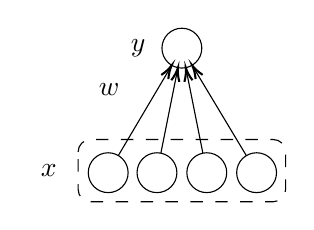
\begin{tikzpicture}[x=0.75pt,y=0.75pt,yscale=-1,xscale=1]
%uncomment if require: \path (0,146); %set diagram left start at 0, and has height of 146

%Rounded Rect [id:dp492723450593467]
\draw  [dash pattern={on 4.5pt off 4.5pt}] (120,86) .. controls (120,82.69) and (122.69,80) .. (126,80) -- (214,80) .. controls (217.31,80) and (220,82.69) .. (220,86) -- (220,104) .. controls (220,107.31) and (217.31,110) .. (214,110) -- (126,110) .. controls (122.69,110) and (120,107.31) .. (120,104) -- cycle ;

% Text Node
\draw    (134.5, 96) circle [x radius= 9.6, y radius= 9.6]   ;
\draw (134.5,96) node   [align=left] {\begin{minipage}[lt]{8.67pt}\setlength\topsep{0pt}

\end{minipage}};
% Text Node
\draw    (158, 96) circle [x radius= 9.6, y radius= 9.6]   ;
\draw (158,96) node   [align=left] {\begin{minipage}[lt]{8.67pt}\setlength\topsep{0pt}

\end{minipage}};
% Text Node
\draw    (182, 96) circle [x radius= 9.6, y radius= 9.6]   ;
\draw (182,96) node   [align=left] {\begin{minipage}[lt]{8.67pt}\setlength\topsep{0pt}

\end{minipage}};
% Text Node
\draw    (206, 96) circle [x radius= 9.6, y radius= 9.6]   ;
\draw (206,96) node   [align=left] {\begin{minipage}[lt]{8.67pt}\setlength\topsep{0pt}

\end{minipage}};
% Text Node
\draw    (170, 36) circle [x radius= 9.6, y radius= 9.6]   ;
\draw (170,36) node   [align=left] {\begin{minipage}[lt]{8.67pt}\setlength\topsep{0pt}

\end{minipage}};
% Text Node
\draw (105.93,95) node   [align=left] {\begin{minipage}[lt]{8.67pt}\setlength\topsep{0pt}
\begin{center}
$\displaystyle \boldsymbol{x}$
\end{center}

\end{minipage}};
% Text Node
\draw (134.93,56) node   [align=left] {\begin{minipage}[lt]{8.67pt}\setlength\topsep{0pt}
\begin{center}
$\displaystyle \boldsymbol{w}$
\end{center}

\end{minipage}};
% Text Node
\draw (148.93,36) node   [align=left] {\begin{minipage}[lt]{8.67pt}\setlength\topsep{0pt}
\begin{center}
$\displaystyle y$
\end{center}

\end{minipage}};
% Connection
\draw    (139.39,87.73) -- (164.09,45.99) ;
\draw [shift={(165.11,44.27)}, rotate = 480.61] [color={rgb, 255:red, 0; green, 0; blue, 0 }  ][line width=0.75]    (6.56,-1.97) .. controls (4.17,-0.84) and (1.99,-0.18) .. (0,0) .. controls (1.99,0.18) and (4.17,0.84) .. (6.56,1.97)   ;
% Connection
\draw    (159.88,86.58) -- (167.72,47.38) ;
\draw [shift={(168.12,45.42)}, rotate = 461.31] [color={rgb, 255:red, 0; green, 0; blue, 0 }  ][line width=0.75]    (6.56,-1.97) .. controls (4.17,-0.84) and (1.99,-0.18) .. (0,0) .. controls (1.99,0.18) and (4.17,0.84) .. (6.56,1.97)   ;
% Connection
\draw    (180.12,86.58) -- (172.28,47.38) ;
\draw [shift={(171.88,45.42)}, rotate = 438.69] [color={rgb, 255:red, 0; green, 0; blue, 0 }  ][line width=0.75]    (6.56,-1.97) .. controls (4.17,-0.84) and (1.99,-0.18) .. (0,0) .. controls (1.99,0.18) and (4.17,0.84) .. (6.56,1.97)   ;
% Connection
\draw    (201.06,87.76) -- (175.97,45.95) ;
\draw [shift={(174.94,44.24)}, rotate = 419.03999999999996] [color={rgb, 255:red, 0; green, 0; blue, 0 }  ][line width=0.75]    (6.56,-1.97) .. controls (4.17,-0.84) and (1.99,-0.18) .. (0,0) .. controls (1.99,0.18) and (4.17,0.84) .. (6.56,1.97)   ;

\end{tikzpicture}}
        \caption{A neuron.}
        \label{fig:neuron}
    \end{subfigure}
    \begin{subfigure}[b]{0.32\linewidth}
        \centering
        \resizebox{.9\textwidth}{!}{

\tikzset{every picture/.style={line width=0.75pt}} %set default line width to 0.75pt

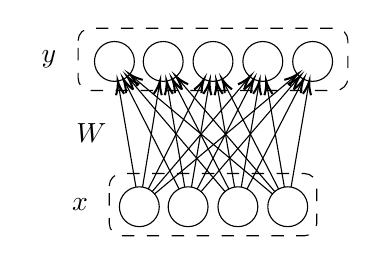
\begin{tikzpicture}[x=0.75pt,y=0.75pt,yscale=-1,xscale=1]
%uncomment if require: \path (0,129); %set diagram left start at 0, and has height of 129

%Rounded Rect [id:dp6663897747680421]
\draw  [dash pattern={on 4.5pt off 4.5pt}] (50,86) .. controls (50,82.69) and (52.69,80) .. (56,80) -- (144,80) .. controls (147.31,80) and (150,82.69) .. (150,86) -- (150,104) .. controls (150,107.31) and (147.31,110) .. (144,110) -- (56,110) .. controls (52.69,110) and (50,107.31) .. (50,104) -- cycle ;
%Rounded Rect [id:dp431982528179069]
\draw  [dash pattern={on 4.5pt off 4.5pt}] (35,16) .. controls (35,12.69) and (37.69,10) .. (41,10) -- (159,10) .. controls (162.31,10) and (165,12.69) .. (165,16) -- (165,34) .. controls (165,37.31) and (162.31,40) .. (159,40) -- (41,40) .. controls (37.69,40) and (35,37.31) .. (35,34) -- cycle ;

% Text Node
\draw    (64.5, 96) circle [x radius= 9.6, y radius= 9.6]   ;
\draw (64.5,96) node   [align=left] {\begin{minipage}[lt]{8.67pt}\setlength\topsep{0pt}

\end{minipage}};
% Text Node
\draw    (88, 96) circle [x radius= 9.6, y radius= 9.6]   ;
\draw (88,96) node   [align=left] {\begin{minipage}[lt]{8.67pt}\setlength\topsep{0pt}

\end{minipage}};
% Text Node
\draw    (112, 96) circle [x radius= 9.6, y radius= 9.6]   ;
\draw (112,96) node   [align=left] {\begin{minipage}[lt]{8.67pt}\setlength\topsep{0pt}

\end{minipage}};
% Text Node
\draw    (136, 96) circle [x radius= 9.6, y radius= 9.6]   ;
\draw (136,96) node   [align=left] {\begin{minipage}[lt]{8.67pt}\setlength\topsep{0pt}

\end{minipage}};
% Text Node
\draw (35.93,95) node   [align=left] {\begin{minipage}[lt]{8.67pt}\setlength\topsep{0pt}
\begin{center}
$\displaystyle \boldsymbol{x}$
\end{center}

\end{minipage}};
% Text Node
\draw (39.93,57) node   [align=left] {\begin{minipage}[lt]{8.67pt}\setlength\topsep{0pt}
\begin{center}
$\displaystyle \boldsymbol{W}$
\end{center}

\end{minipage}};
% Text Node
\draw (20.93,25) node   [align=left] {\begin{minipage}[lt]{8.67pt}\setlength\topsep{0pt}
\begin{center}
$\displaystyle \boldsymbol{y}$
\end{center}

\end{minipage}};
% Text Node
\draw    (52.5, 26) circle [x radius= 9.6, y radius= 9.6]   ;
\draw (52.5,26) node   [align=left] {\begin{minipage}[lt]{8.67pt}\setlength\topsep{0pt}

\end{minipage}};
% Text Node
\draw    (76, 26) circle [x radius= 9.6, y radius= 9.6]   ;
\draw (76,26) node   [align=left] {\begin{minipage}[lt]{8.67pt}\setlength\topsep{0pt}

\end{minipage}};
% Text Node
\draw    (100, 26) circle [x radius= 9.6, y radius= 9.6]   ;
\draw (100,26) node   [align=left] {\begin{minipage}[lt]{8.67pt}\setlength\topsep{0pt}

\end{minipage}};
% Text Node
\draw    (124, 26) circle [x radius= 9.6, y radius= 9.6]   ;
\draw (124,26) node   [align=left] {\begin{minipage}[lt]{8.67pt}\setlength\topsep{0pt}

\end{minipage}};
% Text Node
\draw    (148, 26) circle [x radius= 9.6, y radius= 9.6]   ;
\draw (148,26) node   [align=left] {\begin{minipage}[lt]{8.67pt}\setlength\topsep{0pt}

\end{minipage}};
% Connection
\draw    (62.88,86.53) -- (54.46,37.44) ;
\draw [shift={(54.12,35.47)}, rotate = 440.27] [color={rgb, 255:red, 0; green, 0; blue, 0 }  ][line width=0.75]    (6.56,-1.97) .. controls (4.17,-0.84) and (1.99,-0.18) .. (0,0) .. controls (1.99,0.18) and (4.17,0.84) .. (6.56,1.97)   ;
% Connection
\draw    (66.06,86.52) -- (74.12,37.45) ;
\draw [shift={(74.44,35.48)}, rotate = 459.33] [color={rgb, 255:red, 0; green, 0; blue, 0 }  ][line width=0.75]    (6.56,-1.97) .. controls (4.17,-0.84) and (1.99,-0.18) .. (0,0) .. controls (1.99,0.18) and (4.17,0.84) .. (6.56,1.97)   ;
% Connection
\draw    (68.85,87.43) -- (94.75,36.35) ;
\draw [shift={(95.65,34.57)}, rotate = 476.89] [color={rgb, 255:red, 0; green, 0; blue, 0 }  ][line width=0.75]    (6.56,-1.97) .. controls (4.17,-0.84) and (1.99,-0.18) .. (0,0) .. controls (1.99,0.18) and (4.17,0.84) .. (6.56,1.97)   ;
% Connection
\draw    (70.72,88.68) -- (116.48,34.84) ;
\draw [shift={(117.78,33.32)}, rotate = 490.36] [color={rgb, 255:red, 0; green, 0; blue, 0 }  ][line width=0.75]    (6.56,-1.97) .. controls (4.17,-0.84) and (1.99,-0.18) .. (0,0) .. controls (1.99,0.18) and (4.17,0.84) .. (6.56,1.97)   ;
% Connection
\draw    (71.86,89.83) -- (139.11,33.46) ;
\draw [shift={(140.64,32.17)}, rotate = 500.03] [color={rgb, 255:red, 0; green, 0; blue, 0 }  ][line width=0.75]    (6.56,-1.97) .. controls (4.17,-0.84) and (1.99,-0.18) .. (0,0) .. controls (1.99,0.18) and (4.17,0.84) .. (6.56,1.97)   ;
% Connection
\draw    (83.65,87.43) -- (57.75,36.35) ;
\draw [shift={(56.85,34.57)}, rotate = 423.11] [color={rgb, 255:red, 0; green, 0; blue, 0 }  ][line width=0.75]    (6.56,-1.97) .. controls (4.17,-0.84) and (1.99,-0.18) .. (0,0) .. controls (1.99,0.18) and (4.17,0.84) .. (6.56,1.97)   ;
% Connection
\draw    (86.38,86.53) -- (77.96,37.44) ;
\draw [shift={(77.62,35.47)}, rotate = 440.27] [color={rgb, 255:red, 0; green, 0; blue, 0 }  ][line width=0.75]    (6.56,-1.97) .. controls (4.17,-0.84) and (1.99,-0.18) .. (0,0) .. controls (1.99,0.18) and (4.17,0.84) .. (6.56,1.97)   ;
% Connection
\draw    (89.62,86.53) -- (98.04,37.44) ;
\draw [shift={(98.38,35.47)}, rotate = 459.73] [color={rgb, 255:red, 0; green, 0; blue, 0 }  ][line width=0.75]    (6.56,-1.97) .. controls (4.17,-0.84) and (1.99,-0.18) .. (0,0) .. controls (1.99,0.18) and (4.17,0.84) .. (6.56,1.97)   ;
% Connection
\draw    (92.39,87.46) -- (118.69,36.32) ;
\draw [shift={(119.61,34.54)}, rotate = 477.22] [color={rgb, 255:red, 0; green, 0; blue, 0 }  ][line width=0.75]    (6.56,-1.97) .. controls (4.17,-0.84) and (1.99,-0.18) .. (0,0) .. controls (1.99,0.18) and (4.17,0.84) .. (6.56,1.97)   ;
% Connection
\draw    (94.25,88.71) -- (140.45,34.81) ;
\draw [shift={(141.75,33.29)}, rotate = 490.6] [color={rgb, 255:red, 0; green, 0; blue, 0 }  ][line width=0.75]    (6.56,-1.97) .. controls (4.17,-0.84) and (1.99,-0.18) .. (0,0) .. controls (1.99,0.18) and (4.17,0.84) .. (6.56,1.97)   ;
% Connection
\draw    (105.78,88.68) -- (60.02,34.84) ;
\draw [shift={(58.72,33.32)}, rotate = 409.64] [color={rgb, 255:red, 0; green, 0; blue, 0 }  ][line width=0.75]    (6.56,-1.97) .. controls (4.17,-0.84) and (1.99,-0.18) .. (0,0) .. controls (1.99,0.18) and (4.17,0.84) .. (6.56,1.97)   ;
% Connection
\draw    (107.61,87.46) -- (81.31,36.32) ;
\draw [shift={(80.39,34.54)}, rotate = 422.78] [color={rgb, 255:red, 0; green, 0; blue, 0 }  ][line width=0.75]    (6.56,-1.97) .. controls (4.17,-0.84) and (1.99,-0.18) .. (0,0) .. controls (1.99,0.18) and (4.17,0.84) .. (6.56,1.97)   ;
% Connection
\draw    (110.38,86.53) -- (101.96,37.44) ;
\draw [shift={(101.62,35.47)}, rotate = 440.27] [color={rgb, 255:red, 0; green, 0; blue, 0 }  ][line width=0.75]    (6.56,-1.97) .. controls (4.17,-0.84) and (1.99,-0.18) .. (0,0) .. controls (1.99,0.18) and (4.17,0.84) .. (6.56,1.97)   ;
% Connection
\draw    (113.62,86.53) -- (122.04,37.44) ;
\draw [shift={(122.38,35.47)}, rotate = 459.73] [color={rgb, 255:red, 0; green, 0; blue, 0 }  ][line width=0.75]    (6.56,-1.97) .. controls (4.17,-0.84) and (1.99,-0.18) .. (0,0) .. controls (1.99,0.18) and (4.17,0.84) .. (6.56,1.97)   ;
% Connection
\draw    (116.39,87.46) -- (142.69,36.32) ;
\draw [shift={(143.61,34.54)}, rotate = 477.22] [color={rgb, 255:red, 0; green, 0; blue, 0 }  ][line width=0.75]    (6.56,-1.97) .. controls (4.17,-0.84) and (1.99,-0.18) .. (0,0) .. controls (1.99,0.18) and (4.17,0.84) .. (6.56,1.97)   ;
% Connection
\draw    (128.64,89.83) -- (61.39,33.46) ;
\draw [shift={(59.86,32.17)}, rotate = 399.97] [color={rgb, 255:red, 0; green, 0; blue, 0 }  ][line width=0.75]    (6.56,-1.97) .. controls (4.17,-0.84) and (1.99,-0.18) .. (0,0) .. controls (1.99,0.18) and (4.17,0.84) .. (6.56,1.97)   ;
% Connection
\draw    (129.75,88.71) -- (83.55,34.81) ;
\draw [shift={(82.25,33.29)}, rotate = 409.4] [color={rgb, 255:red, 0; green, 0; blue, 0 }  ][line width=0.75]    (6.56,-1.97) .. controls (4.17,-0.84) and (1.99,-0.18) .. (0,0) .. controls (1.99,0.18) and (4.17,0.84) .. (6.56,1.97)   ;
% Connection
\draw    (131.61,87.46) -- (105.31,36.32) ;
\draw [shift={(104.39,34.54)}, rotate = 422.78] [color={rgb, 255:red, 0; green, 0; blue, 0 }  ][line width=0.75]    (6.56,-1.97) .. controls (4.17,-0.84) and (1.99,-0.18) .. (0,0) .. controls (1.99,0.18) and (4.17,0.84) .. (6.56,1.97)   ;
% Connection
\draw    (134.38,86.53) -- (125.96,37.44) ;
\draw [shift={(125.62,35.47)}, rotate = 440.27] [color={rgb, 255:red, 0; green, 0; blue, 0 }  ][line width=0.75]    (6.56,-1.97) .. controls (4.17,-0.84) and (1.99,-0.18) .. (0,0) .. controls (1.99,0.18) and (4.17,0.84) .. (6.56,1.97)   ;
% Connection
\draw    (137.62,86.53) -- (146.04,37.44) ;
\draw [shift={(146.38,35.47)}, rotate = 459.73] [color={rgb, 255:red, 0; green, 0; blue, 0 }  ][line width=0.75]    (6.56,-1.97) .. controls (4.17,-0.84) and (1.99,-0.18) .. (0,0) .. controls (1.99,0.18) and (4.17,0.84) .. (6.56,1.97)   ;

\end{tikzpicture}}
        \caption{A layer.}
        \label{fig:layer}
    \end{subfigure}
    \begin{subfigure}[b]{0.32\linewidth}
        \centering
        \resizebox{.9\textwidth}{!}{

\tikzset{every picture/.style={line width=0.75pt}} %set default line width to 0.75pt

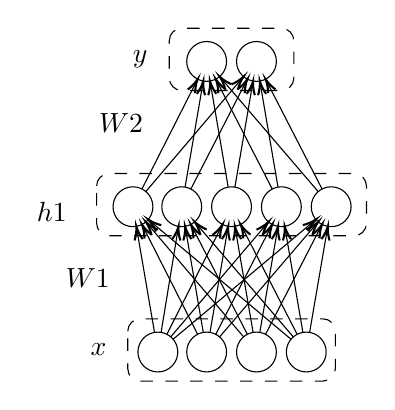
\begin{tikzpicture}[x=0.75pt,y=0.75pt,yscale=-1,xscale=1]
%uncomment if require: \path (0,300); %set diagram left start at 0, and has height of 300

%Rounded Rect [id:dp06623654071530738]
\draw  [dash pattern={on 4.5pt off 4.5pt}] (70,196) .. controls (70,192.69) and (72.69,190) .. (76,190) -- (164,190) .. controls (167.31,190) and (170,192.69) .. (170,196) -- (170,214) .. controls (170,217.31) and (167.31,220) .. (164,220) -- (76,220) .. controls (72.69,220) and (70,217.31) .. (70,214) -- cycle ;
%Rounded Rect [id:dp029839322386400635]
\draw  [dash pattern={on 4.5pt off 4.5pt}] (55,126) .. controls (55,122.69) and (57.69,120) .. (61,120) -- (179,120) .. controls (182.31,120) and (185,122.69) .. (185,126) -- (185,144) .. controls (185,147.31) and (182.31,150) .. (179,150) -- (61,150) .. controls (57.69,150) and (55,147.31) .. (55,144) -- cycle ;
%Rounded Rect [id:dp1895454286656968]
\draw  [dash pattern={on 4.5pt off 4.5pt}] (90,56) .. controls (90,52.69) and (92.69,50) .. (96,50) -- (144,50) .. controls (147.31,50) and (150,52.69) .. (150,56) -- (150,74) .. controls (150,77.31) and (147.31,80) .. (144,80) -- (96,80) .. controls (92.69,80) and (90,77.31) .. (90,74) -- cycle ;

% Text Node
\draw    (84.5, 206) circle [x radius= 9.6, y radius= 9.6]   ;
\draw (84.5,206) node   [align=left] {\begin{minipage}[lt]{8.67pt}\setlength\topsep{0pt}

\end{minipage}};
% Text Node
\draw    (108, 206) circle [x radius= 9.6, y radius= 9.6]   ;
\draw (108,206) node   [align=left] {\begin{minipage}[lt]{8.67pt}\setlength\topsep{0pt}

\end{minipage}};
% Text Node
\draw    (132, 206) circle [x radius= 9.6, y radius= 9.6]   ;
\draw (132,206) node   [align=left] {\begin{minipage}[lt]{8.67pt}\setlength\topsep{0pt}

\end{minipage}};
% Text Node
\draw    (156, 206) circle [x radius= 9.6, y radius= 9.6]   ;
\draw (156,206) node   [align=left] {\begin{minipage}[lt]{8.67pt}\setlength\topsep{0pt}

\end{minipage}};
% Text Node
\draw (55.93,205) node   [align=left] {\begin{minipage}[lt]{8.67pt}\setlength\topsep{0pt}
\begin{center}
$\displaystyle \boldsymbol{x}$
\end{center}

\end{minipage}};
% Text Node
\draw (46,167) node   [align=left] {\begin{minipage}[lt]{8.67pt}\setlength\topsep{0pt}
\begin{center}
$\displaystyle \LayerMatrix{W}{1}$
\end{center}

\end{minipage}};
% Text Node
\draw (32,135) node   [align=left] {\begin{minipage}[lt]{8.67pt}\setlength\topsep{0pt}
\begin{center}
$\displaystyle \LayerVector{h}{1}$
\end{center}

\end{minipage}};
% Text Node
\draw    (72.5, 136) circle [x radius= 9.6, y radius= 9.6]   ;
\draw (72.5,136) node   [align=left] {\begin{minipage}[lt]{8.67pt}\setlength\topsep{0pt}

\end{minipage}};
% Text Node
\draw    (96, 136) circle [x radius= 9.6, y radius= 9.6]   ;
\draw (96,136) node   [align=left] {\begin{minipage}[lt]{8.67pt}\setlength\topsep{0pt}

\end{minipage}};
% Text Node
\draw    (120, 136) circle [x radius= 9.6, y radius= 9.6]   ;
\draw (120,136) node   [align=left] {\begin{minipage}[lt]{8.67pt}\setlength\topsep{0pt}

\end{minipage}};
% Text Node
\draw    (144, 136) circle [x radius= 9.6, y radius= 9.6]   ;
\draw (144,136) node   [align=left] {\begin{minipage}[lt]{8.67pt}\setlength\topsep{0pt}

\end{minipage}};
% Text Node
\draw    (168, 136) circle [x radius= 9.6, y radius= 9.6]   ;
\draw (168,136) node   [align=left] {\begin{minipage}[lt]{8.67pt}\setlength\topsep{0pt}

\end{minipage}};
% Text Node
\draw    (108, 66) circle [x radius= 9.6, y radius= 9.6]   ;
\draw (108,66) node   [align=left] {\begin{minipage}[lt]{8.67pt}\setlength\topsep{0pt}

\end{minipage}};
% Text Node
\draw    (132, 66) circle [x radius= 9.6, y radius= 9.6]   ;
\draw (132,66) node   [align=left] {\begin{minipage}[lt]{8.67pt}\setlength\topsep{0pt}

\end{minipage}};
% Text Node
\draw (61.93,92) node   [align=left] {\begin{minipage}[lt]{8.67pt}\setlength\topsep{0pt}
\begin{center}
$\displaystyle \LayerMatrix{W}{2}$
\end{center}

\end{minipage}};
% Text Node
\draw (75.93,65) node   [align=left] {\begin{minipage}[lt]{8.67pt}\setlength\topsep{0pt}
\begin{center}
$\displaystyle \Vector{y}$
\end{center}

\end{minipage}};
% Connection
\draw    (82.88,196.53) -- (74.46,147.44) ;
\draw [shift={(74.12,145.47)}, rotate = 440.27] [color={rgb, 255:red, 0; green, 0; blue, 0 }  ][line width=0.75]    (6.56,-1.97) .. controls (4.17,-0.84) and (1.99,-0.18) .. (0,0) .. controls (1.99,0.18) and (4.17,0.84) .. (6.56,1.97)   ;
% Connection
\draw    (86.06,196.52) -- (94.12,147.45) ;
\draw [shift={(94.44,145.48)}, rotate = 459.33] [color={rgb, 255:red, 0; green, 0; blue, 0 }  ][line width=0.75]    (6.56,-1.97) .. controls (4.17,-0.84) and (1.99,-0.18) .. (0,0) .. controls (1.99,0.18) and (4.17,0.84) .. (6.56,1.97)   ;
% Connection
\draw    (88.85,197.43) -- (114.75,146.35) ;
\draw [shift={(115.65,144.57)}, rotate = 476.89] [color={rgb, 255:red, 0; green, 0; blue, 0 }  ][line width=0.75]    (6.56,-1.97) .. controls (4.17,-0.84) and (1.99,-0.18) .. (0,0) .. controls (1.99,0.18) and (4.17,0.84) .. (6.56,1.97)   ;
% Connection
\draw    (90.72,198.68) -- (136.48,144.84) ;
\draw [shift={(137.78,143.32)}, rotate = 490.36] [color={rgb, 255:red, 0; green, 0; blue, 0 }  ][line width=0.75]    (6.56,-1.97) .. controls (4.17,-0.84) and (1.99,-0.18) .. (0,0) .. controls (1.99,0.18) and (4.17,0.84) .. (6.56,1.97)   ;
% Connection
\draw    (91.86,199.83) -- (159.11,143.46) ;
\draw [shift={(160.64,142.17)}, rotate = 500.03] [color={rgb, 255:red, 0; green, 0; blue, 0 }  ][line width=0.75]    (6.56,-1.97) .. controls (4.17,-0.84) and (1.99,-0.18) .. (0,0) .. controls (1.99,0.18) and (4.17,0.84) .. (6.56,1.97)   ;
% Connection
\draw    (103.65,197.43) -- (77.75,146.35) ;
\draw [shift={(76.85,144.57)}, rotate = 423.11] [color={rgb, 255:red, 0; green, 0; blue, 0 }  ][line width=0.75]    (6.56,-1.97) .. controls (4.17,-0.84) and (1.99,-0.18) .. (0,0) .. controls (1.99,0.18) and (4.17,0.84) .. (6.56,1.97)   ;
% Connection
\draw    (106.38,196.53) -- (97.96,147.44) ;
\draw [shift={(97.62,145.47)}, rotate = 440.27] [color={rgb, 255:red, 0; green, 0; blue, 0 }  ][line width=0.75]    (6.56,-1.97) .. controls (4.17,-0.84) and (1.99,-0.18) .. (0,0) .. controls (1.99,0.18) and (4.17,0.84) .. (6.56,1.97)   ;
% Connection
\draw    (109.62,196.53) -- (118.04,147.44) ;
\draw [shift={(118.38,145.47)}, rotate = 459.73] [color={rgb, 255:red, 0; green, 0; blue, 0 }  ][line width=0.75]    (6.56,-1.97) .. controls (4.17,-0.84) and (1.99,-0.18) .. (0,0) .. controls (1.99,0.18) and (4.17,0.84) .. (6.56,1.97)   ;
% Connection
\draw    (112.39,197.46) -- (138.69,146.32) ;
\draw [shift={(139.61,144.54)}, rotate = 477.22] [color={rgb, 255:red, 0; green, 0; blue, 0 }  ][line width=0.75]    (6.56,-1.97) .. controls (4.17,-0.84) and (1.99,-0.18) .. (0,0) .. controls (1.99,0.18) and (4.17,0.84) .. (6.56,1.97)   ;
% Connection
\draw    (114.25,198.71) -- (160.45,144.81) ;
\draw [shift={(161.75,143.29)}, rotate = 490.6] [color={rgb, 255:red, 0; green, 0; blue, 0 }  ][line width=0.75]    (6.56,-1.97) .. controls (4.17,-0.84) and (1.99,-0.18) .. (0,0) .. controls (1.99,0.18) and (4.17,0.84) .. (6.56,1.97)   ;
% Connection
\draw    (125.78,198.68) -- (80.02,144.84) ;
\draw [shift={(78.72,143.32)}, rotate = 409.64] [color={rgb, 255:red, 0; green, 0; blue, 0 }  ][line width=0.75]    (6.56,-1.97) .. controls (4.17,-0.84) and (1.99,-0.18) .. (0,0) .. controls (1.99,0.18) and (4.17,0.84) .. (6.56,1.97)   ;
% Connection
\draw    (127.61,197.46) -- (101.31,146.32) ;
\draw [shift={(100.39,144.54)}, rotate = 422.78] [color={rgb, 255:red, 0; green, 0; blue, 0 }  ][line width=0.75]    (6.56,-1.97) .. controls (4.17,-0.84) and (1.99,-0.18) .. (0,0) .. controls (1.99,0.18) and (4.17,0.84) .. (6.56,1.97)   ;
% Connection
\draw    (130.38,196.53) -- (121.96,147.44) ;
\draw [shift={(121.62,145.47)}, rotate = 440.27] [color={rgb, 255:red, 0; green, 0; blue, 0 }  ][line width=0.75]    (6.56,-1.97) .. controls (4.17,-0.84) and (1.99,-0.18) .. (0,0) .. controls (1.99,0.18) and (4.17,0.84) .. (6.56,1.97)   ;
% Connection
\draw    (133.62,196.53) -- (142.04,147.44) ;
\draw [shift={(142.38,145.47)}, rotate = 459.73] [color={rgb, 255:red, 0; green, 0; blue, 0 }  ][line width=0.75]    (6.56,-1.97) .. controls (4.17,-0.84) and (1.99,-0.18) .. (0,0) .. controls (1.99,0.18) and (4.17,0.84) .. (6.56,1.97)   ;
% Connection
\draw    (136.39,197.46) -- (162.69,146.32) ;
\draw [shift={(163.61,144.54)}, rotate = 477.22] [color={rgb, 255:red, 0; green, 0; blue, 0 }  ][line width=0.75]    (6.56,-1.97) .. controls (4.17,-0.84) and (1.99,-0.18) .. (0,0) .. controls (1.99,0.18) and (4.17,0.84) .. (6.56,1.97)   ;
% Connection
\draw    (148.64,199.83) -- (81.39,143.46) ;
\draw [shift={(79.86,142.17)}, rotate = 399.97] [color={rgb, 255:red, 0; green, 0; blue, 0 }  ][line width=0.75]    (6.56,-1.97) .. controls (4.17,-0.84) and (1.99,-0.18) .. (0,0) .. controls (1.99,0.18) and (4.17,0.84) .. (6.56,1.97)   ;
% Connection
\draw    (149.75,198.71) -- (103.55,144.81) ;
\draw [shift={(102.25,143.29)}, rotate = 409.4] [color={rgb, 255:red, 0; green, 0; blue, 0 }  ][line width=0.75]    (6.56,-1.97) .. controls (4.17,-0.84) and (1.99,-0.18) .. (0,0) .. controls (1.99,0.18) and (4.17,0.84) .. (6.56,1.97)   ;
% Connection
\draw    (151.61,197.46) -- (125.31,146.32) ;
\draw [shift={(124.39,144.54)}, rotate = 422.78] [color={rgb, 255:red, 0; green, 0; blue, 0 }  ][line width=0.75]    (6.56,-1.97) .. controls (4.17,-0.84) and (1.99,-0.18) .. (0,0) .. controls (1.99,0.18) and (4.17,0.84) .. (6.56,1.97)   ;
% Connection
\draw    (154.38,196.53) -- (145.96,147.44) ;
\draw [shift={(145.62,145.47)}, rotate = 440.27] [color={rgb, 255:red, 0; green, 0; blue, 0 }  ][line width=0.75]    (6.56,-1.97) .. controls (4.17,-0.84) and (1.99,-0.18) .. (0,0) .. controls (1.99,0.18) and (4.17,0.84) .. (6.56,1.97)   ;
% Connection
\draw    (157.62,196.53) -- (166.04,147.44) ;
\draw [shift={(166.38,145.47)}, rotate = 459.73] [color={rgb, 255:red, 0; green, 0; blue, 0 }  ][line width=0.75]    (6.56,-1.97) .. controls (4.17,-0.84) and (1.99,-0.18) .. (0,0) .. controls (1.99,0.18) and (4.17,0.84) .. (6.56,1.97)   ;
% Connection
\draw    (76.85,127.43) -- (102.75,76.35) ;
\draw [shift={(103.65,74.57)}, rotate = 476.89] [color={rgb, 255:red, 0; green, 0; blue, 0 }  ][line width=0.75]    (6.56,-1.97) .. controls (4.17,-0.84) and (1.99,-0.18) .. (0,0) .. controls (1.99,0.18) and (4.17,0.84) .. (6.56,1.97)   ;
% Connection
\draw    (78.72,128.68) -- (124.48,74.84) ;
\draw [shift={(125.78,73.32)}, rotate = 490.36] [color={rgb, 255:red, 0; green, 0; blue, 0 }  ][line width=0.75]    (6.56,-1.97) .. controls (4.17,-0.84) and (1.99,-0.18) .. (0,0) .. controls (1.99,0.18) and (4.17,0.84) .. (6.56,1.97)   ;
% Connection
\draw    (97.62,126.53) -- (106.04,77.44) ;
\draw [shift={(106.38,75.47)}, rotate = 459.73] [color={rgb, 255:red, 0; green, 0; blue, 0 }  ][line width=0.75]    (6.56,-1.97) .. controls (4.17,-0.84) and (1.99,-0.18) .. (0,0) .. controls (1.99,0.18) and (4.17,0.84) .. (6.56,1.97)   ;
% Connection
\draw    (100.39,127.46) -- (126.69,76.32) ;
\draw [shift={(127.61,74.54)}, rotate = 477.22] [color={rgb, 255:red, 0; green, 0; blue, 0 }  ][line width=0.75]    (6.56,-1.97) .. controls (4.17,-0.84) and (1.99,-0.18) .. (0,0) .. controls (1.99,0.18) and (4.17,0.84) .. (6.56,1.97)   ;
% Connection
\draw    (118.38,126.53) -- (109.96,77.44) ;
\draw [shift={(109.62,75.47)}, rotate = 440.27] [color={rgb, 255:red, 0; green, 0; blue, 0 }  ][line width=0.75]    (6.56,-1.97) .. controls (4.17,-0.84) and (1.99,-0.18) .. (0,0) .. controls (1.99,0.18) and (4.17,0.84) .. (6.56,1.97)   ;
% Connection
\draw    (121.62,126.53) -- (130.04,77.44) ;
\draw [shift={(130.38,75.47)}, rotate = 459.73] [color={rgb, 255:red, 0; green, 0; blue, 0 }  ][line width=0.75]    (6.56,-1.97) .. controls (4.17,-0.84) and (1.99,-0.18) .. (0,0) .. controls (1.99,0.18) and (4.17,0.84) .. (6.56,1.97)   ;
% Connection
\draw    (139.61,127.46) -- (113.31,76.32) ;
\draw [shift={(112.39,74.54)}, rotate = 422.78] [color={rgb, 255:red, 0; green, 0; blue, 0 }  ][line width=0.75]    (6.56,-1.97) .. controls (4.17,-0.84) and (1.99,-0.18) .. (0,0) .. controls (1.99,0.18) and (4.17,0.84) .. (6.56,1.97)   ;
% Connection
\draw    (142.38,126.53) -- (133.96,77.44) ;
\draw [shift={(133.62,75.47)}, rotate = 440.27] [color={rgb, 255:red, 0; green, 0; blue, 0 }  ][line width=0.75]    (6.56,-1.97) .. controls (4.17,-0.84) and (1.99,-0.18) .. (0,0) .. controls (1.99,0.18) and (4.17,0.84) .. (6.56,1.97)   ;
% Connection
\draw    (161.75,128.71) -- (115.55,74.81) ;
\draw [shift={(114.25,73.29)}, rotate = 409.4] [color={rgb, 255:red, 0; green, 0; blue, 0 }  ][line width=0.75]    (6.56,-1.97) .. controls (4.17,-0.84) and (1.99,-0.18) .. (0,0) .. controls (1.99,0.18) and (4.17,0.84) .. (6.56,1.97)   ;
% Connection
\draw    (163.61,127.46) -- (137.31,76.32) ;
\draw [shift={(136.39,74.54)}, rotate = 422.78] [color={rgb, 255:red, 0; green, 0; blue, 0 }  ][line width=0.75]    (6.56,-1.97) .. controls (4.17,-0.84) and (1.99,-0.18) .. (0,0) .. controls (1.99,0.18) and (4.17,0.84) .. (6.56,1.97)   ;

\end{tikzpicture}}
        \caption{A MLP.}
        \label{fig:mlp}
    \end{subfigure}
    \caption{({\scriptsize A}) An example of a neural network layer. The superscript above the units indicates the layer they belong to. ({\scriptsize A}) A Multi-Layer Perceptron
    with $L=3$ layers (biases not shown). The arrows indicate the flow of forward propagation.}
\end{figure*}

The number of layers and the dimension of their parameter matrices constitute the \emph{architecture} of the network. Network architecture, and the nature of the activation function of the hidden layers, play a major role in determining the kinds of functions a \gls{nn} can learn. Specifically, \glspl{nn} with at least one hidden layer with non-linear activation function (also called \glspl{mlp}, such as the one shown in Figure \ref{fig:mlp}) are \emph{universal approximators}, meaning that they can approximate arbitrarily well any computable function \citep{cybenko1998approximationuniversal}. However, no guarantees as to which kinds of architectures work best can be given, according to the \quotes{no free lungh theorem} \citep{wolpert1997freelunchtheorem}; thus, network architecture is task-dependent and must be optimized with model selection. As regards the activation functions, modern neural networks are commonly trained with three non-linear activation functions (or variations thereof)for which universal approximation capabilities have been proved:
\begin{itemize}
    \item the \emph{sigmoid function}, defined as:
    $$\sigmoid(x) = \frac{1}{1 + e^{-x}};$$
    \item the \emph{hyperbolic tangent function}, defined as:
    $$\tanh(x) = \frac{e^x - e^{-x}}{e^x + e^{-x}};$$
    \item the \gls{relu} function \citep{glorot2011relu}, defined as:
    $$\relu(x) = \max(0, x).$$
    Notice that, even though the \gls{relu} function is not differentiable at $x = 0$, it can be used in practical settings with some adaptation.
\end{itemize}
These three activation functions, and their derivaties, are shown in Figure \ref{fig:activations}.

$x = 0$, it can be used in practical settings with some adaptation.
\begin{figure*}[h!]
    \begin{subfigure}[b]{0.32\linewidth}
        \centering
        \resizebox{.8\textwidth}{!}{\begin{tikzpicture}[declare function={sigma(\x)=1/(1+exp(-\x));
sigmap(\x)=sigma(\x)*(1-sigma(\x));}]
\begin{axis}%
[
    % grid=major,     
    xmin=-6,
    xmax=6,
    axis x line=bottom,
    ytick={-1,-.5,0,.5,1},
    ymax=1.1,
    axis y line=middle,
    samples=200,
    domain=-6:6,
    width=\textwidth,
    height=.6\textwidth,
    scale only axis=true,
    %legend style={at={(.4,.9)}}  
]
    \addplot[mark=none]   (x,{sigma(x)});
    \addplot[dashed,mark=none]   (x,{sigmap(x)});
    %\legend{$\sigma(x)$,$\sigma'(x)$}
\end{axis}
\end{tikzpicture}}
        \caption{Sigmoid}
        \label{fig:sigmoid}
    \end{subfigure}
    \begin{subfigure}[b]{0.32\linewidth}
        \centering
        \resizebox{.8\textwidth}{!}{\begin{tikzpicture}[declare function={tanhp(\x)=1-tanh(\x)^2;}]
\begin{axis}%
[
    % grid=major,     
    xmin=-4.1,
    xmax=4.1,
    axis x line=middle,
    ytick={-1,0,1},
    ymax=1.1,
    ymin=-1.1,
    axis y line=middle,
    samples=200,
    domain=-4:4,
    width=\textwidth,
    height=.8\textwidth,
    scale only axis=true,
    %legend style={at={(.3,.9)}}      
]
    \addplot[mark=none]   (x,{tanh(\x)});
    \addplot[dashed,mark=none]   (x,{tanhp(\x)});
    %\legend{$\Fun{tanh}(x)$,$\Fun{tanh}'(x)$}
\end{axis}
\end{tikzpicture}}
        \caption{Hyperbolic Tangent}
        \label{fig:hyptan}
    \end{subfigure}
    \begin{subfigure}[b]{0.32\linewidth}
        \centering
        \resizebox{.8\textwidth}{!}{\begin{tikzpicture}[declare function={
    relu(\x)=max(0,\x);
    relup(\x)=(\x<0) * (0) + (\x>0) * (1);
}]
\begin{axis}%
[
    % grid=major,     
    xmin=-2.1,
    xmax=2.1,
    xtick={-2,0,2},
    axis x line=bottom,
    ytick={0,1,2},
    ymax=2.2,
    axis y line=middle,
    samples=200,
    domain=-2:2,
    width=\textwidth,
    height=.6\textwidth,
    scale only axis=true,
    %legend style={at={(.4,.9)}}     
]
    \addplot[mark=none]   (x,{relu(\x)});
    \foreach \xStart/\xEnd  in {-2/-0.001, 0.001/2} {
        \addplot[domain=\xStart:\xEnd,dashed] {relup(x)};
    }
    %\addplot[red,dashed,mark=none]   (x,{relup(x)});
    %\legend{$\Fun{ReLU}(x)$,$\Fun{ReLU}'(x)$}
\end{axis}
\end{tikzpicture}}
        \caption{Rectified Linear Unit}
        \label{fig:relu}
    \end{subfigure}
    \caption{Examples of activation functions for the hidden layers (solid line) and their derivatives (dashed line).}
    \label{fig:activations}
\end{figure*}
One distinctive advantage of \glspl{nn} with respect to other learning algorithms is \emph{automatic feature engineering}: in fact, the hidden layers of a \gls{nn} extract features from the data without an explicit guidance from the end user. This means that the network itself decides which \keyword{representation} of the data is relevant to solve a given task by tuning the parameters during learning; this decision is driven by the high-level goal of approximating the input-output relationship of interest. This ability is crucial in tasks where knowledge is difficult to represent, or where there is not enough domain expertise to manually devise features, and has been the key of the success of \glspl{nn} in \gls{ml}.

\subsection{Training}\label{sec:training}
Learning in a \gls{nn} requires several passes through the training set. Each pass is called an \emph{epoch}, and consists of two phases. In the first phase, called \emph{forward propagation}, training examples are fed to the network, which produces an output for each data point. Subsequently, the error between the output and the target is calculated by the loss function. The second phase consists in propagating the error back to the hidden layers to calculate the gradient of the loss function at each layer. This is done via the well-known \keyword{backpropagation} algorithm \citep{rumelhart1986backprop}, which is basically an application of the chain rule of derivation for function composition. Once the gradient of the loss function is available at each layer, the parameters are modified using the \gls{sgd} update rule. Training \glspl{nn} requires particular care to ensure the convergence of the \gls{sgd} algorithm. In particular, the initial values of the weight matrices should be initialized with small random values around 0 for \emph{simmetry breaking}, and the learning rate must be $< 1$, to prevent too large update steps which would make the objective function diverge from the local minima \citep{lecun1998backprop}.

\subsection{Output Layers and Loss Functions}\label{sec:loss}
The output layer of a \gls{nn} is chosen according to the task it should learn. In turn, each task is associated to a specific loss function that must be minimized by the optimizer, in order to find a set of parameters that generalize. \glspl{nn} are usually trained with \gls{mle} \citep{hastie2009elements}. Specifically, one assumes that the unknown function $\Target$ is a distribution $p(y\given\Vector{x})$, whose parameters are given by the neural network. The idea is to make this distribution match the distribution of the data observed through a dataset $\Data = \Set{(\PatternVector{x}{i}, \Pattern{y}{i})}_{i=1}^n$. This corresponds to minimizing the dissimilarity between the distribution parameterized by the network and the empirical distribution of the data. This dissimilarity can be quantified by the \gls{kld} between the empirical distribution and the distribution parameterized by the neural network:
$$\KLD{p_{\mathrm{data}}}{p} = \Expect_{(\Vector{x}, y) \sim p_{\mathrm{data}}}\Brack{\log p_{\mathrm{data}}(y \given \Vector{x}) - \log p(y \given \Vector{x})},$$
where $p_{\mathrm{data}}$ is the empirical distribution. The \gls{kld} is a proper loss function, since its output is always $\ge 0$, and it is 0 if and only if $p_{\mathrm{data}} = p$. Thus, we can minimize it under the \gls{erm} principle. Since $p_{\mathrm{data}}$ does not depend on the parameters of $p(y \given \Vector{x})$, to minimize the \gls{kld} it is sufficient to minimize the term $- \Expect_{(\Vector{x}, y) \sim p_{\mathrm{data}}}\Brack{\log p(y \given \Vector{x})}$, \ie the negative log-likelihood of the distribution parameterized by the network:
$$\argmin_{\Param} \frac{1}{n} \sum_{i=1}^n -\log p(\Pattern{y}{i} \given \PatternVector{x}{i}),$$
where $\Param$ are the parameters of the network as usual. Below, we detail about three of the most common output layers, and the loss functions by which the corresponding networks can be trained. Following, we assume a dataset $\Data$ defined as above, and a neural network with parameters $\Param$ and $L$ layers for simplicity.

\paragraph{Linear Output Layer}
A linear output layer is used to solve regression tasks, \ie tasks where the output space is continuous. Assuming a neural network with $L$ layers, a linear output layer is defined as:

$$\Layer{f}{L}(\LayerVector{h}{L-1}) = \LayerMatrix{W}{L} \LayerVector{h}{L-1} + \LayerVector{b}{L}.$$
Notice that a linear output layer does not have an activation function; equivalently, one can think that the activation function is the identity. The model assumed for the true conditional is the following:
$$p(y \given \Vector{x}) \sim \Normal{f(\Vector{x})}{1}.$$
In other words, the network outputs the mean of a Gaussian distribution with unit variance. Applying the \gls{mle}, minimizing the \gls{kld} is equivalent to minimizing the \gls{mse} loss function:
$$\Loss(\Param, (\Vector{x}, y)) =\Fun{MSE}(\Vector{x}, y) \defeq \norm{\hat{y} - y}_2,$$
where $\hat{y} = f(\Vector{x}) \in \Real$ is the output of the network for a particular data point $\Vector{x}$.
Notice that minimizing the \gls{mse} corresponds to minimizing the Euclidean distance between the target $y$ and the prediction of the network $f(\Vector{x})$. A network with only one single linear output layer trained to minimize the \gls{mse} loss function is commonly known in \gls{ml} literature as the Linear Regression model.

\paragraph{Logistic Output Layer}
A logistic output layer is used to solve binary classification tasks, \ie tasks where the output space is the discrete set $\Set{0, 1}$. The label 0 is usually called the \emph{negative} class, while the label 1 is called \emph{positive}. The layer is defined as follows:

$$\Layer{f}{L}(\LayerVector{h}{L-1}) = \sigmoid \Par{\LayerMatrix{W}{L} \LayerVector{h}{L-1} + \LayerVector{b}{L}}.$$
Since the codomain of the sigmoid function is the real-valued interval $(0, 1) \subset \Real$, it is suitable to express output probabilities. To apply \gls{mle} to a binary classification task, the following model for the true conditional is assumed:
$$p(y \given \Vector{x}) \sim \Fun{Bernoulli}(f(\Vector{x})),$$
In other words, the neural network outputs the parameter of a Bernoulli distribution for each data point $\Vector{x}$. Using \gls{mle}, minimizing the \gls{kld} is equivalent to minimizing the \gls{bce} loss function:
$$\Loss(\Param, (\Vector{x}, y)) = \Fun{BCE}(\Vector{x},y) \defeq y\, \log(\hat{y}) + ( 1 - y) \log(1 - \hat{y}),$$
where $\hat{y} = f(\Vector{x})$ as usual. Training a single logistic output layer with the \gls{bce} loss function is equivalent to training a Logistic Regression model.

\paragraph{Softmax Output Layer}
The softmax output layer is used in multi-class classification tasks, \ie tasks where the output space is a discrete set $\Cal{C} = \Set{c_1, \ldots, c_k}$ of $k$ mutually exclusive classes. In this cases, the targets $y$ are expressed as \emph{one-hot} vectors $\Vector{y} \in \Real^k$. In practice, each position of the one-hot vector corresponds to a specific class, and its entries are defined as follows:
\begin{align*}
    \Vector{y}_i=
    \begin{cases}
        1 & \mathrm{if}\; y = c_i\\
        0 & \mathrm{otherwise}.
    \end{cases}
\end{align*}
In words, a one-hot vector encodes the target as a discrete probability distribution over the possible classes, where all the mass is put on the class corresponding to the label $y$. The layer is defined as:

$$\Layer{f}{L}(\LayerVector{h}{L-1}) = \softmax \Par{\LayerMatrix{W}{L} \LayerVector{h}{L-1} + \LayerVector{b}{L}},$$
where the \emph{softmax} activation function is defined element-wise over a generic vector $\Vector{s} \in \Real^k$ as:
$$\softmax(\Vector{s}_i) = \frac{e^{\Vector{s}_i}}{\sum_{j=1}^k e^{\Vector{s}_j}}.$$
In practice, a softmax layer outputs a score for each possible class, and the vector of scores is normalized to be a probability distribution by the softmax function. The model for the true conditional assumed in this case is the following:
$$p(y \given \Vector{x}) \sim \Fun{Multinoulli}_k(f_{\Param}(\Vector{x})).$$
In other words, the conditional is a Multinoulli (categorical) distribution for the $k$ classes, and the network outputs its parameters (the probabilities for each class). Minimizing the \gls{kld} in this setting is equivalent to minimizing the \gls{ce} loss function:
$$\Loss(\Param, (\Vector{x}, y)) = \mathrm{CE}(\Vector{x}, y) \defeq - \sum_{i=1}^k \Vector{y}_i \log \Vector{\hat{y}}_i,$$
where $\Vector{\hat{y}} = f(\Vector{x})$ is the output distribution as given the network. Notice that the \gls{bce} loss function is just a special case of \gls{ce} where $k = 2$. A \gls{nn} with one single softmax output trained with \gls{ce} is known in the \gls{ml} literature as the Softmax Regression model.

\subsection{Regularization}\label{sec:regularization}
As we have briefly described in Section \ref{sec:learning}, regularizing a \gls{ml} model requires to somehow limit the complexity of the hypotheses space, such that the learning algorithm is more likely to select hypotheses that do not overfit the training data. For \glspl{nn}, one straightforward approach to limit complexity is to reduce the number of hidden layers, and the number of units in each layer. Other strategies are discussed below.

\paragraph{Penalized Loss Function}
One very general regularization technique, which is not restricted to \glspl{nn}, is to impose a \emph{preference bias} to the possible values the weights might take, such that configurations that generalize achieve a lower training error than configurations that overfit. Focusing again on the supervised case, and assuming a dataset $\Data = \Set{(\PatternVector{x}{i}, \Pattern{y}{i})}_{i=1}^n$ as usual, this can be achieved by augmenting the training ojective with a \emph{penalty term} as follows:
$$\argmin_{\Param} \frac{1}{n} \sum_{i=1}^n \Loss(\Param, (\PatternVector{x}{i}, \Pattern{y}{i})) + \lambda\norm{\Param}_p,$$
where $\norm{.}_p$ indicates a generic $p$-norm. The norm of the parameters implement the preference criteria used to avoid overfitting, whose influence on the training objective is controlled by a hyper-parameter $\lambda$. Depending on the value of $p$, we distinguish:
\begin{itemize}
    \item L1 regularization, where $p=1$. The bias of L1 regularization is to push the values of some weights to zero. This corresponds to training a \gls{nn} with less parameters (parameters set to 0 do not contribute to the loss function);
    \item L2 regularization, where $p=2$. The bias induced of L2 regularization is to penalize large values of the weights. Intuitively, restricting the range of the values that the weights can take limits the type of functions the network can approximate.
\end{itemize}
Notice that these are not the only penalties possible, although they are the most used in practical settings \citep{hastie2009elements}.

\paragraph{Early Stopping}
Early stopping \citep{prechelt1998earlystopping} is another general regularization scheme, which is widely adopted in \glspl{nn} training. In short, it requires monitoring a performance metric (which can be the value of the loss function or other task-specific metrics) on the validation set, in order to stop the learning process as soon as overfitting is detected. Once learning has stopped, the parameters that yielded the best score according to the metric are chosen by the learning algorithm. Intuitively, early stopping implicitly biases the hypotheses space by limiting the number of training iterations, which in turn limits the number of hypotheses evaluated during training.

\paragraph{Dropout}
Dropout \citep{srivastava2014dropout} is a regularization technique that is specific to \glspl{nn}. The idea behind dropout is to use a very expressive network for training, whose capacity is constrained stochastically at each iteration of the learning procedure. At each pass through a batch of training data, dropout \quotes{turns off} some of the units in a layer by multiplying their output with a binary vector mask, whose entries are samples from a Bernoulli distribution with hyper-parameter $p_{\mathrm{keep}}$, called \emph{dropout rate}. This has a double effect: first, a smaller number of parameters is used to compute a prediction (because some of them are made ineffective by the binary mask); second, the parameters used by the network are different at each pass (because of the stochasticity of the mask). According to this second implication, dropout implements a dynamic form of \emph{model ensembling}, a \gls{ml} technique in which one combines several low-capacity model to obtain a stronger predictor.

\section{Auto-Encoders}
An \gls{ae} \citep{baldi2012autoenc} is a \gls{nn} architecture for unsupervised learning. \glspl{ae} are trained to reconstruct their inputs by jointly learning two mappings, one from the input space to a \keyword{latent space}, and another from the latent space back to the input space. During training, the latent space learns general features about the input that help achieve a good reconstruction. Given a $d$-dimensional input vector $\Vector{x} \in \Real^d$, an autoencoder computes a function $f(\Vector{x}) = (\EncoderNet \circ \DecoderNet)(\Vector{x})$ as follows:
\begin{align*}
    \Vector{h} &= \EncoderNet(\Vector{x})\\
    \Vector{r} &= \DecoderNet(\Vector{h}),
\end{align*}
where $\Vector{h} \in \Real^h$ is an $h$-dimensional \emph{latent code}, $\Vector{r} \in \Real^d$ is a \emph{reconstruction} of the input, $\EncoderNet$ is an encoding \gls{nn} or \keyword{encoder} with parameters $\EncParam$, $\DecoderNet$ is a decoding \gls{nn} or \keyword{decoder}, with parameters $\DecParam$, and $\Param = (\EncParam, \DecParam)$. Despite being an unsupervised model, \glspl{ae} can be trained in a supervised way, by implicitly using a dataset of the form $\Data = \Set{(\PatternVector{x}{i}, \PatternVector{x}{i})}_{i=1}^n$, \ie one where the input itself is the target. The loss function of an \gls{ae} is called \emph{reconstruction loss}, and measures the error between the input $\Vector{x}$ and the reconstructed output $f(\Vector{x})$, as shown in Figure \ref{fig:autoencoder}. For continuous inputs, the reconstruction is simply the \gls{mse} loss:
$$\Loss(\Param, (\Vector{x}, \Vector{r})) = \Norm{\Vector{x}-\Vector{r}}_2,$$
while for discrete inputs the \gls{ce} can be used instead.

\begin{figure*}[h!]
    \centering
    \resizebox{.45\textwidth}{!}{

\tikzset{every picture/.style={line width=0.75pt}} %set default line width to 0.75pt        

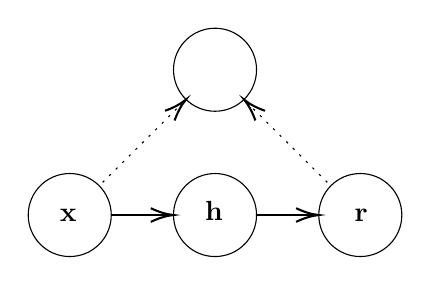
\begin{tikzpicture}[x=0.75pt,y=0.75pt,yscale=-1,xscale=1]
%uncomment if require: \path (0,148); %set diagram left start at 0, and has height of 148

%Shape: Boxed Line [id:dp8923577175434361] 
\draw  [dash pattern={on 0.84pt off 2.51pt}]  (70,110) -- (124.54,55.81) ;
\draw [shift={(125.96,54.4)}, rotate = 495.18] [color={rgb, 255:red, 0; green, 0; blue, 0 }  ][line width=0.75]    (10.93,-3.29) .. controls (6.95,-1.4) and (3.31,-0.3) .. (0,0) .. controls (3.31,0.3) and (6.95,1.4) .. (10.93,3.29)   ;
%Shape: Boxed Line [id:dp9855569745062982] 
\draw  [dash pattern={on 0.84pt off 2.51pt}]  (209.96,110) -- (155.42,55.81) ;
\draw [shift={(154,54.4)}, rotate = 404.82] [color={rgb, 255:red, 0; green, 0; blue, 0 }  ][line width=0.75]    (10.93,-3.29) .. controls (6.95,-1.4) and (3.31,-0.3) .. (0,0) .. controls (3.31,0.3) and (6.95,1.4) .. (10.93,3.29)   ;
%Shape: Circle [id:dp5965402013258883] 
\draw   (120,110) .. controls (120,98.95) and (128.95,90) .. (140,90) .. controls (151.05,90) and (160,98.95) .. (160,110) .. controls (160,121.05) and (151.05,130) .. (140,130) .. controls (128.95,130) and (120,121.05) .. (120,110) -- cycle ;
%Shape: Circle [id:dp24273838994586128] 
\draw  [fill={rgb, 255:red, 255; green, 255; blue, 255 }  ,fill opacity=1 ] (50,110) .. controls (50,98.95) and (58.95,90) .. (70,90) .. controls (81.05,90) and (90,98.95) .. (90,110) .. controls (90,121.05) and (81.05,130) .. (70,130) .. controls (58.95,130) and (50,121.05) .. (50,110) -- cycle ;
%Shape: Circle [id:dp07818860842911124] 
\draw  [fill={rgb, 255:red, 255; green, 255; blue, 255 }  ,fill opacity=1 ] (190,110) .. controls (190,98.95) and (198.95,90) .. (210,90) .. controls (221.05,90) and (230,98.95) .. (230,110) .. controls (230,121.05) and (221.05,130) .. (210,130) .. controls (198.95,130) and (190,121.05) .. (190,110) -- cycle ;
%Shape: Circle [id:dp6286535373530038] 
\draw   (120,40) .. controls (120,28.95) and (128.95,20) .. (140,20) .. controls (151.05,20) and (160,28.95) .. (160,40) .. controls (160,51.05) and (151.05,60) .. (140,60) .. controls (128.95,60) and (120,51.05) .. (120,40) -- cycle ;
%Straight Lines [id:da3987012470307014] 
\draw    (90,110) -- (118,110) ;
\draw [shift={(120,110)}, rotate = 180] [color={rgb, 255:red, 0; green, 0; blue, 0 }  ][line width=0.75]    (10.93,-3.29) .. controls (6.95,-1.4) and (3.31,-0.3) .. (0,0) .. controls (3.31,0.3) and (6.95,1.4) .. (10.93,3.29)   ;
%Straight Lines [id:da5505317995787229] 
\draw    (160,110) -- (188,110) ;
\draw [shift={(190,110)}, rotate = 180] [color={rgb, 255:red, 0; green, 0; blue, 0 }  ][line width=0.75]    (10.93,-3.29) .. controls (6.95,-1.4) and (3.31,-0.3) .. (0,0) .. controls (3.31,0.3) and (6.95,1.4) .. (10.93,3.29)   ;

% Text Node
\draw (134,102) node [anchor=north west][inner sep=0.75pt]    {$\mathbf{h}$};
% Text Node
\draw (64,106) node [anchor=north west][inner sep=0.75pt]    {$\mathbf{x}$};
% Text Node
\draw (206,106) node [anchor=north west][inner sep=0.75pt]    {$\mathbf{r}$};
% Text Node
\draw (133,33) node [anchor=north west][inner sep=0.75pt]    {$\Loss$};


\end{tikzpicture}}
    \caption{An Auto-Encoder.}
    \label{fig:autoencoder}
\end{figure*}
If the latent space of the \gls{ae} is not constrained in any way, it learns to just copy its input to the output: in fact, one can always have $\Vector{x} = \Vector{r}$ everywhere by choosing $f$ as the identity function. This is not very useful in practice, as a network structured in this way would not learn anything useful about the data; thus, many forms of structuring or constraining the latent space have been studied. Perhaps the simplest form of \gls{ae} is the undercomplete \gls{ae}, \ie one where $h < d$. In this case, the latent space acts like a \emph{bottleneck} that is forced to retain relevant features that allow to reconstruct the input, while discarding irrelevant ones. A useful byproduct of training an undercomplete \gls{ae} is that the latent space acts as a \emph{manifold}, \ie a lower-dimensional subspace with Euclidean properties where data points are projected onto. One limitation of this kind of architecture is that one has to choose the capacity of the encoder and decoder very carefully. As an extreme case, consider that an over-capacitated \gls{ae} with a 1-D latent space could learn to map each data point to the set of integers. Clearly, this mapping would be uninformative of the true data distribution.

\subsection{Regularized Auto-Encoders}
Regularized \glspl{ae} generally use $h \geq d$, but impose constraints on the representations learned by the latent space through penalties on the loss function. Specifically, a regularized \gls{ae} optimizes the following loss function:

$$\Loss(\Param, (\Vector{x}, \Vector{r})) + \lambda \Psi(\Vector{h}),$$
where different choices of $\Psi$ define different variants. For example, \emph{sparse} AEs
are trained in such a way that the latent space produces sparse representations, meaning that only certain units are active for certain data inputs. This can be accomplished by constraining the mean activation of the units to be small. Specifically, in a sparse \gls{ae}, if $\rho \in \Real$ is a desired average activation of the outputs $\Vector{h} \in \Real^h$ of a hidden layer, the penalty is formulated as:
$$\Psi(\Vector{h}) = \sum_{i=1}^h \rho \log \frac{\rho}{\Vector{h}_i} (1 - \rho) \log \frac{1-\rho}{1-\Vector{h}_i}.$$
If $\rho$ is chosen to be small, the penalty constrains most hidden units to have zero activation. Similarly, \emph{contractive} \glspl{ae} \citep{rifai2011contractiveautoenc} regularize the objective function by imposing a penalty on the gradients of the hidden units with respect to the input. More in detail, the penalty term of a contractive \gls{ae} is the following:
$$\Psi(\Vector{h}) = \sum_{i=1}^h\norm{\grad_{\Vector{x}}\Vector{h}_i}_2,$$
which intuitively corresponds to penalizing hidden activations that have large variation for small variations in the input. Thus, the local structure of the latent space is forced to be smooth. Differently from the other variants, \emph{denoising} \glspl{ae} \citep{vincent2010denoisingautoenc} achieve regularization acting on the training procedure, rather than via a penalty term. In a denoising \gls{ae}, the input $\Vector{x}$ is corrupted before being passed to the network (usually through Gaussian noise addition). Thus, the network uses the corrupted version $\tilde{\Vector{x}}$ during forward propagation, while the loss is calculated on the original input. By being trained to remove the noise from the input, the network is forced to learn meaningful patterns. The forward propagation phase of a denoising \gls{ae} is shown in Figure \ref{fig:denoising-ae}.
\begin{figure*}[h!]
    \centering
    \resizebox{.6\textwidth}{!}{

\tikzset{every picture/.style={line width=0.75pt}} %set default line width to 0.75pt        

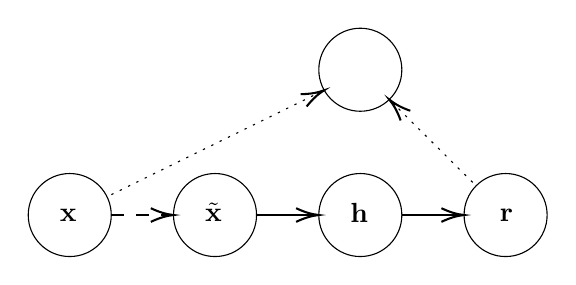
\begin{tikzpicture}[x=0.75pt,y=0.75pt,yscale=-1,xscale=1]
%uncomment if require: \path (0,300); %set diagram left start at 0, and has height of 300

%Straight Lines [id:da8399576495369319] 
\draw  [dash pattern={on 0.84pt off 2.51pt}]  (140,130) -- (260.72,70.8) ;
\draw [shift={(262.52,69.92)}, rotate = 513.88] [color={rgb, 255:red, 0; green, 0; blue, 0 }  ][line width=0.75]    (10.93,-3.29) .. controls (6.95,-1.4) and (3.31,-0.3) .. (0,0) .. controls (3.31,0.3) and (6.95,1.4) .. (10.93,3.29)   ;
%Shape: Boxed Line [id:dp10887462373342993] 
\draw  [dash pattern={on 0.84pt off 2.51pt}]  (349.96,130) -- (295.42,75.81) ;
\draw [shift={(294,74.4)}, rotate = 404.82] [color={rgb, 255:red, 0; green, 0; blue, 0 }  ][line width=0.75]    (10.93,-3.29) .. controls (6.95,-1.4) and (3.31,-0.3) .. (0,0) .. controls (3.31,0.3) and (6.95,1.4) .. (10.93,3.29)   ;
%Shape: Circle [id:dp5603710113663563] 
\draw   (260,130) .. controls (260,118.95) and (268.95,110) .. (280,110) .. controls (291.05,110) and (300,118.95) .. (300,130) .. controls (300,141.05) and (291.05,150) .. (280,150) .. controls (268.95,150) and (260,141.05) .. (260,130) -- cycle ;
%Shape: Circle [id:dp44224070274078864] 
\draw  [fill={rgb, 255:red, 255; green, 255; blue, 255 }  ,fill opacity=1 ] (190,130) .. controls (190,118.95) and (198.95,110) .. (210,110) .. controls (221.05,110) and (230,118.95) .. (230,130) .. controls (230,141.05) and (221.05,150) .. (210,150) .. controls (198.95,150) and (190,141.05) .. (190,130) -- cycle ;
%Shape: Circle [id:dp9930956365882191] 
\draw  [fill={rgb, 255:red, 255; green, 255; blue, 255 }  ,fill opacity=1 ] (330,130) .. controls (330,118.95) and (338.95,110) .. (350,110) .. controls (361.05,110) and (370,118.95) .. (370,130) .. controls (370,141.05) and (361.05,150) .. (350,150) .. controls (338.95,150) and (330,141.05) .. (330,130) -- cycle ;
%Shape: Circle [id:dp530216459507133] 
\draw   (260,60) .. controls (260,48.95) and (268.95,40) .. (280,40) .. controls (291.05,40) and (300,48.95) .. (300,60) .. controls (300,71.05) and (291.05,80) .. (280,80) .. controls (268.95,80) and (260,71.05) .. (260,60) -- cycle ;
%Straight Lines [id:da7671516825865974] 
\draw    (230,130) -- (258,130) ;
\draw [shift={(260,130)}, rotate = 180] [color={rgb, 255:red, 0; green, 0; blue, 0 }  ][line width=0.75]    (10.93,-3.29) .. controls (6.95,-1.4) and (3.31,-0.3) .. (0,0) .. controls (3.31,0.3) and (6.95,1.4) .. (10.93,3.29)   ;
%Straight Lines [id:da7943056265648183] 
\draw    (300,130) -- (328,130) ;
\draw [shift={(330,130)}, rotate = 180] [color={rgb, 255:red, 0; green, 0; blue, 0 }  ][line width=0.75]    (10.93,-3.29) .. controls (6.95,-1.4) and (3.31,-0.3) .. (0,0) .. controls (3.31,0.3) and (6.95,1.4) .. (10.93,3.29)   ;
%Shape: Circle [id:dp3989296686115751] 
\draw  [fill={rgb, 255:red, 255; green, 255; blue, 255 }  ,fill opacity=1 ] (120,130) .. controls (120,118.95) and (128.95,110) .. (140,110) .. controls (151.05,110) and (160,118.95) .. (160,130) .. controls (160,141.05) and (151.05,150) .. (140,150) .. controls (128.95,150) and (120,141.05) .. (120,130) -- cycle ;
%Straight Lines [id:da8399844169636741] 
\draw  [dash pattern={on 4.5pt off 4.5pt}]  (160,130) -- (188,130) ;
\draw [shift={(190,130)}, rotate = 180] [color={rgb, 255:red, 0; green, 0; blue, 0 }  ][line width=0.75]    (10.93,-3.29) .. controls (6.95,-1.4) and (3.31,-0.3) .. (0,0) .. controls (3.31,0.3) and (6.95,1.4) .. (10.93,3.29)   ;

% Text Node
\draw (134,126) node [anchor=north west][inner sep=0.75pt]    {$\mathbf{x}$};

% Text Node
\draw (204,123) node [anchor=north west][inner sep=0.75pt]    {$\tilde{\mathbf{x}}$};
% Text Node
\draw (274,123) node [anchor=north west][inner sep=0.75pt]    {$\mathbf{h}$};
% Text Node
\draw (346,126) node [anchor=north west][inner sep=0.75pt]    {$\mathbf{r}$};
% Text Node
\draw (273,52) node [anchor=north west][inner sep=0.75pt]    {$\Loss$};



\end{tikzpicture}}
    \caption{A denoising Auto-Encoder. The dashed arrow indicates the corruption process which transforms the input $\Vector{x}$ into a noisy version $\tilde{\Vector{x}}$, which is not directly part of the forward propagation.}
    \label{fig:denoising-ae}
\end{figure*}

\section{Deep Learning}
In Section \ref{sec:nn}, we have talked about the representational power of \glspl{nn}. However, the way this representational power is attained is greatly influenced by the \emph{depth} of the network, \ie its number of layers. When a \gls{nn} is \quotes{deep}, the hidden features are organized during learning in a hierarchy, in which simpler features of the early layers are progressively combined into very sophisticated features in subsequent layers. Although \quotes{shallow} networks (networks with very few but large hidden layers) have their same approximating capabilities, deep networks combine features in a more computationally efficient way \citep{bengio2009deeparch}. This data-driven \emph{representational bias} has proven effective in many practical domains, such as computer vision \citep{krizhevsky2017imagenet} and \gls{nlp} \citep{vaswani2017transformer}, establishing the success of deep \glspl{nn} in many \gls{ml} tasks. The term \gls{dl} \citep{goodfellow2016dl}, coined around 2006, is used to refer to \gls{nn} architectures composed of a large number of hidden layers, usually $\geq 3$. The representational power of deep networks comes in hand with a number of computational challenges that arise from their depth. Below, we summarize the most well-known:
\begin{itemize}
    \item the loss functions used for training deep networks are extremely complicated and non-convex, since the hidden layers have non-linear activation functions. This means that gradient-based methods may get stuck in bad local minima;
    \item very deep networks suffer from \emph{vanishing} or \emph{exploding gradient} issues, which can prevent the network from learning, or make the optimization numerically unstable, respectively;
    \item training deep \glspl{nn} requires large datasets and an extensive amount of computational power.
\end{itemize}
These three major issues have been the focus of basic research on deep networks in the last years. As regards the first challenge, these problems have been tackled by better characterizing the properties of the optimization problem \glspl{nn} try to solve \citep{goodfellow2015optimization,janocha2017lossfunction}. In parallel, improvements have been achieved by devising more effective optimizers \citep{kingma2015adam,ruder2016overviewsgd} and effective activation functions \citep{glorot2011relu}. As regards the second challenge, several mechanisms to prevent the two undesirable phenomena from happening have been proposed and applied with success; the most known are gradient clipping \citep{zhang2020gradientclipping} to prevent gradient explosion, batch normalization \citep{ioffe2015batchnorm} and residual connections \citep{he2016resnets} to prevent gradient vanishing. As for the third challenge, major contributions came from the advent of the big data revolution, which ensured large and progressively more curated data sources, and the use of \gls{gpu} vectorization, automatic differentiation and computational graphs \citep{abadi2016tensorflow,paszke2017pytorch} to speed up the training and inference processes of deep networks.

\subsection{Convolutional Neural Networks}
A \gls{cnn} \citep{lecun1995convolutionalnn} is a kind of \gls{nn} born in the field of computer vision. The development of \glspl{cnn} started long before the \quotes{deep learning renaissance} in 2006, but they only recently became popular, after demonstrating their effectiveness in several image recognition tasks \citep{krizhevsky2017imagenet}. Given their historical importance in the landscape of \gls{dl}, we shall present them briefly even though they are not part of this thesis. The standard hidden layer of a \gls{cnn} is called \emph{convolutional layer}, and it is able to process 2-dimensional data such as images. It does so with parameterized \emph{filters} which are applied to an input through a convolution operation. The output of a filter is usually called \emph{feature map}. More in detail, a 2-D convolutional filter computes computes a feature map where each entry is defined as follows:
$$\Matrix{F}_{ij} = (\Matrix{M} * \Matrix{K})_{ij} = \sum_{i=1}^{w} \sum_{j=1}^{h} \Matrix{M}_{(i+s)(j+t)}\Matrix{K}_{st}.$$
In the equation above, $\Matrix{M} \in \Real^{w \times h}$ is a 2-D matrix (for example, an image with width $w$ and height $h$), $\Matrix{K} \in \Real^{s \times t}$ is a learnable filter, or \emph{kernel}, with width $s \ll w$ and height $t \ll h$, and $*$ is a convolutional operator. In practice, the filter is \quotes{slid} on the input row-wise. The values in the feature map have larger magnitude if parts of the input match the filter, or more intuitively, if the pattern of the filter is detected (to some extent) in the input image. In turn, this implies that each feature of the feature map shares the same weights (those of the kernel). This approach is called \emph{weight sharing}, and it implements \emph{translational invariance}, \ie features are detected regardless of their position in the input. Another essential layer of \glspl{cnn} is a \emph{pooling layer}. It works by dividing the input in non-overlapping regions, and computing an aggregation function (usually a max) for each region. Pooling serves a double purpose: firstly, it reduces the number of weights needed in subsequent layers, thus maintaining computational tractability as the depth of the network grows; secondly, it acts as a regularizer, as it discards the specific information of the region where it is applied, picking up only one representative pattern. Convolutional and pooling layers are applied sequentially to the input data, followed by a standard hidden layer activation function, usually a ReLU. The three layers (Convolution-Pooling-ReLU) in cascade are the standard building block of convolutional architectures. The last layers of a \gls{cnn} usually consist of a standard \gls{mlp} (or a single output layer), which uses the final representation computed by the convolutional blocks as input, and computes the corresponding task-dependent output. Even though they were born within the computer vision field, \glspl{cnn} have been generalized to 1-D inputs (such as sound waves in \emph{speech recognition} tasks) and 3-D inputs (such as video frames in \emph{object tracking} tasks).

\section{Deep Generative Models}\label{sec:dgm}
Typical unsupervised tasks require to learn the probability distribution of the data, or some aspect of it, such as, for example, how the data is clustered together. Broadly speaking, the two operations that approximating the data distribution allows are:
\begin{itemize}
    \item \keyword{inference}, that is, computing the density of arbitrary data points;
    \item \keyword{sampling}, that is, generating new data by drawing samples from the distribution.
\end{itemize}
\glspl{dgm} \citep{goodfellow2016dl} are essentially deep architectures that learn how to do inference and sampling, or just sampling, from the data distribution. Based on this definition, we can further distinguish between:
\begin{itemize}
    \item \emph{prescribed} \glspl{dgm}, which can jointly learn inference as well as sampling;
    \item \emph{implicit} \glspl{dgm}, which only learn sampling.
\end{itemize}
Below, we provide a brief overview on the topic.

\subsection{Prescribed Deep Generative Models}\label{sec:autoregressive}
Prescribed models are trained under the \gls{mle} principle, by minimizing the \gls{kld} between the empirical data distribution $p_{\mathrm{data}}$ and a model $p_{\Param}$ of the true data distribution parameterized by a deep \gls{nn} with parameters $\Param$:
$$\argmin_{\Param} \KLD{p}{p_{\Param}} \defeq \Expect_{\Vector{x} \sim p_{\mathrm{data}}}\Brack{\log p_{\mathrm{data}}(\Vector{x}) -\log p_{\Param}(\Vector{x})}.$$
Notice that the setup is slightly different from Section \ref{sec:loss}: there, the neural network was estimating the parameters of a conditional distribution; here, it is approximating the distribution itself. As seen before, the term $\log p_{\mathrm{data}}(\Vector{x})$ does not depend on the parameters of the model; thus, the following quantity can be minimized equivalently:
$$\argmin_{\Param} \Expect_{\Vector{x} \sim p}\Brack{-\log p_{\Param}(\Vector{x})}.$$
In practice, applying \gls{mle} on a (generally unlabelled) dataset $\Data = \Set{\PatternVector{x}{i}}_{i=1}^n$, prescribed \glspl{dgm} learn the data distribution by minimizing the negative log-likelihood of the observed data using \gls{sgd}:
$$\argmin_{\Param} \frac{1}{n} \sum_{i=1}^n -\log p_{\Param}(\PatternVector{x}{i}).$$
Two prescribed \glspl{dgm} of relevance to this thesis is are described in the following. Besides those mentioned above, other prescribed \glspl{dgm} include for example Sigmoid Belief Networks \citep{neal1992sigmoidbeliefnet}, and Flow-based models \citep{rezende2015normalizingflows}.

\subsubsection*{Autoregressive Models}
An \gls{ar} model is a prescribed \gls{dgm} where the data distribution is decomposed in a product of conditionals according the chain rule of probability:
$$-\log p(\Vector{x}) = -\log\Par{\prod_i p(x_i \given x_{<i})} = \sum_i -\log p(x_i \given x_{<i}),$$
where $x_i$ are random variables, and $x_{<i} = \Par{x_1, x_2, \ldots, x_{i-1}}$. Basically, each conditional is approximated by a deep \gls{nn} $p_{\Param_i}$ that takes as input $x_{<i}$ (which for now we assume to be a fixed-size vector for simplicity) and outputs a distribution over $x_i$. Inference in autoregressive models is achieved by forward propagating the input through each network in the order established by the decomposition, and summing up the intermediate probabilities. To generate a data point according to the learned distribution, it is sufficient to sample each conditional in the order given by the chain rule decomposition. Given their sequentiality, autoregressive models are often implemented with Recurrent Neural Networks (see Section \ref{sec:rnns}); but in principle, any neural network that takes two inputs (the current input of the conditional $x_i$ and a summarization of $x_{<i}$) can be used. Another family of autoregressive models use neural networks with \emph{masking} techniques to constrain their output to follow a given chain rule order. For example, the model by \cite{germain2015made} uses autoencoders, while \cite{vandenoord2016wavenet} uses convolutional layers.

\subsubsection*{Variational Auto-Encoders}
A \gls{vae} \citep{kingma2014vae} is a prescribed \glspl{dgm} which originates from the family of \emph{latent variable models}. In latent variable models, a set of latent variables $\Vector{z} \in \Real^z$, also called explaining factors, is incorporated to the data distribution by marginalization as follows:
$$p(\Vector{x}) = \int p(\Vector{x} \given \Vector{z})\, q(\Vector{z})\, d\Vector{z}.$$
In the above formula, $p(\Vector{x} \given \Vector{z})$ is a \emph{decoding distribution} and $q(\Vector{z})$ is a prior over the latent variables, usually chosen to be a tractable distribution such as a Gaussian. The generative process expressed by a latent variable model consists in sampling from the prior a \quotes{specification} of the data, provided by the latent variables, which is used to condition the decoding distribution. Since the latent variables are not known in general, \glspl{vae} introduce an \emph{encoding distribution} $q(\Vector{z} \given \Vector{x})$ to produce latent variables given a data point. Instead of the data log-likelihood, \glspl{vae} work with a related quantity, called \gls{elbo} of the true log-likelihood, defined as follows:

$$\Fun{ELBO}(\Vector{x}) = \Expect_{\Vector{z} \sim q(\Vector{z} \given \Vector{x})}\Brack{\log p(\Vector{x} \given \Vector{z})} - \KLD{q(\Vector{z} \given \Vector{x})}{q(\Vector{z})},$$
and such that $\log p(\Vector{x}) \geq \Fun{ELBO}(\Vector{x})$. By maximizing the \gls{elbo}, the true log-likelihood of the data can be recovered. Intuitively, this can be achieved by maximizing the expected log-likelihood of the decoding distribution $p(\Vector{x} \given \Vector{z})$ under the encoding distribution (the first term), while making the encoding distribution $q(\Vector{z} \given \Vector{x})$ close to the prior distribution $q(\Vector{z})$ at the same time (as specified by the \gls{kld} term). In practice, $q(\Vector{z})$ is chosen to be a standard Gaussian $\Normal{\ZeroVector}{\Matrix{i}}$ with unit covariance matrix $\Matrix{i}$. The encoder distribution $q(\Vector{z} \given \Vector{x})$ is also a Gaussian distribution, whose mean and standard deviation are given by two different neural networks (which share some parameters but not the output layers). Specifically,
$\Encoder(\Vector{z} \given \Vector{x}) = \Normal{\MeanVec}{\StdVec}$ with $\MeanVec,\StdVec \in \Real^z$, such that $\MeanVec = f(\Vector{x})$, $\StdVec = g(\Vector{x})$. The fact that both the prior and the encoder distributions are Gaussian gives the \gls{kld} term of the \gls{elbo} in closed form. The decoding distribution $p(\Vector{x} \given \Vector{z})$ is implemented as another deep \gls{nn} $\Decoder$ with parameters $\Param$. The loss function minimized by a \gls{vae} is thus the following:
$$\Loss((\Param, \EncParam), \Vector{x}) = - \log \Decoder(\Vector{x} \given \Vector{z}) + \KLD{\Encoder(\Vector{z} \given \Vector{x})}{\Normal{\ZeroVector}{\Matrix{i}}},$$
with $\Vector{z} \sim \Encoder(\Vector{z} \given \Vector{x})$. The leftmost term is a likelihood-based reconstruction loss, and the rightmost term regularizes the encoding distribution by making it similar to the prior. The forward propagation of a \gls{vae} is specified as follows: first, the input $\Vector{x}$ is mapped to the mean and variance of the encoding distribution by the encoder network. The two parameters are used to sample a latent vector $\Vector{z}$. This is turn is given to the decoder network, which outputs a reconstruction $\Vector{r}$. One major issue with this formulation is that this model cannot be trained with \gls{sgd}, since the gradient of a stochastic operation (the sampling from the encoder distribution) is not defined. Thus, the sampling process is reparameterized as $\Normal{\MeanVec}{\StdVec} = \MeanVec + \boldsymbol{\eps}\StdVec$, with $\boldsymbol{\eps} \in \Real^z \sim \Normal{\ZeroVector}{\Matrix{i}}$. This way, the stochastic operation is independent of the input, and gradient backpropagation through the encoder becomes deterministic. The reparameterized model is shown in Figure \ref{fig:vae}.
\begin{figure*}[h!]
    \centering
    \resizebox{.75\textwidth}{!}{

\tikzset{every picture/.style={line width=0.75pt}} %set default line width to 0.75pt

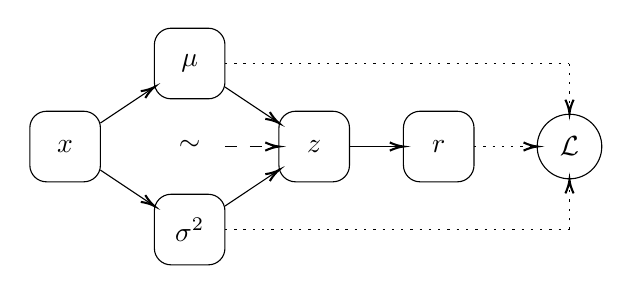
\begin{tikzpicture}[x=0.75pt,y=0.75pt,yscale=-1,xscale=1]
%uncomment if require: \path (0,130); %set diagram left start at 0, and has height of 130

%Straight Lines [id:da06643486433204138]
\draw  [dash pattern={on 0.84pt off 2.51pt}]  (268,20) -- (268,42) ;
\draw [shift={(268,44)}, rotate = 270] [color={rgb, 255:red, 0; green, 0; blue, 0 }  ][line width=0.75]    (6.56,-1.97) .. controls (4.17,-0.84) and (1.99,-0.18) .. (0,0) .. controls (1.99,0.18) and (4.17,0.84) .. (6.56,1.97)   ;
%Straight Lines [id:da6604103885996644]
\draw  [dash pattern={on 0.84pt off 2.51pt}]  (102,20) -- (268,20) ;
%Straight Lines [id:da9796063200949052]
\draw  [dash pattern={on 0.84pt off 2.51pt}]  (268,100) -- (268,78) ;
\draw [shift={(268,76)}, rotate = 450] [color={rgb, 255:red, 0; green, 0; blue, 0 }  ][line width=0.75]    (6.56,-1.97) .. controls (4.17,-0.84) and (1.99,-0.18) .. (0,0) .. controls (1.99,0.18) and (4.17,0.84) .. (6.56,1.97)   ;
%Straight Lines [id:da3305764871838648]
\draw  [dash pattern={on 0.84pt off 2.51pt}]  (102,100) -- (268,100) ;

% Text Node
\draw    (8,51) .. controls (8,46.58) and (11.58,43) .. (16,43) -- (34,43) .. controls (38.42,43) and (42,46.58) .. (42,51) -- (42,69) .. controls (42,73.42) and (38.42,77) .. (34,77) -- (16,77) .. controls (11.58,77) and (8,73.42) .. (8,69) -- cycle  ;
\draw (25,60) node   [align=left] {\begin{minipage}[lt]{20.400000000000002pt}\setlength\topsep{0pt}
\begin{center}
$\displaystyle \boldsymbol{x}$
\end{center}

\end{minipage}};
% Text Node
\draw    (268, 60) circle [x radius= 15.56, y radius= 15.56]   ;
\draw (268,60) node   [align=left] {\begin{minipage}[lt]{13.735995849609345pt}\setlength\topsep{0pt}
\begin{center}
$\displaystyle \mathcal{L}$
\end{center}

\end{minipage}};
% Text Node
\draw    (68,11) .. controls (68,6.58) and (71.58,3) .. (76,3) -- (94,3) .. controls (98.42,3) and (102,6.58) .. (102,11) -- (102,29) .. controls (102,33.42) and (98.42,37) .. (94,37) -- (76,37) .. controls (71.58,37) and (68,33.42) .. (68,29) -- cycle  ;
\draw (85,20) node   [align=left] {\begin{minipage}[lt]{20.400000000000002pt}\setlength\topsep{0pt}
\begin{center}
$\displaystyle \boldsymbol{\mu }$
\end{center}

\end{minipage}};
% Text Node
\draw    (68,91) .. controls (68,86.58) and (71.58,83) .. (76,83) -- (94,83) .. controls (98.42,83) and (102,86.58) .. (102,91) -- (102,109) .. controls (102,113.42) and (98.42,117) .. (94,117) -- (76,117) .. controls (71.58,117) and (68,113.42) .. (68,109) -- cycle  ;
\draw (85,100) node   [align=left] {\begin{minipage}[lt]{20.400000000000002pt}\setlength\topsep{0pt}
\begin{center}
$\displaystyle \boldsymbol{\sigma }^{2}$
\end{center}

\end{minipage}};
% Text Node
\draw    (128,51) .. controls (128,46.58) and (131.58,43) .. (136,43) -- (154,43) .. controls (158.42,43) and (162,46.58) .. (162,51) -- (162,69) .. controls (162,73.42) and (158.42,77) .. (154,77) -- (136,77) .. controls (131.58,77) and (128,73.42) .. (128,69) -- cycle  ;
\draw (145,60) node   [align=left] {\begin{minipage}[lt]{20.400000000000002pt}\setlength\topsep{0pt}
\begin{center}
$\displaystyle \boldsymbol{z}$
\end{center}

\end{minipage}};
% Text Node
\draw    (188,51) .. controls (188,46.58) and (191.58,43) .. (196,43) -- (214,43) .. controls (218.42,43) and (222,46.58) .. (222,51) -- (222,69) .. controls (222,73.42) and (218.42,77) .. (214,77) -- (196,77) .. controls (191.58,77) and (188,73.42) .. (188,69) -- cycle  ;
\draw (205,60) node   [align=left] {\begin{minipage}[lt]{20.400000000000002pt}\setlength\topsep{0pt}
\begin{center}
$\displaystyle \boldsymbol{r}$
\end{center}

\end{minipage}};
% Text Node
\draw (85,60) node   [align=left] {\begin{minipage}[lt]{20.400000000000002pt}\setlength\topsep{0pt}
\begin{center}
$\displaystyle \sim $
\end{center}

\end{minipage}};
% Connection
\draw    (42,48.67) -- (66.34,32.44) ;
\draw [shift={(68,31.33)}, rotate = 506.31] [color={rgb, 255:red, 0; green, 0; blue, 0 }  ][line width=0.75]    (6.56,-1.97) .. controls (4.17,-0.84) and (1.99,-0.18) .. (0,0) .. controls (1.99,0.18) and (4.17,0.84) .. (6.56,1.97)   ;
% Connection
\draw    (42,71.33) -- (66.34,87.56) ;
\draw [shift={(68,88.67)}, rotate = 213.69] [color={rgb, 255:red, 0; green, 0; blue, 0 }  ][line width=0.75]    (6.56,-1.97) .. controls (4.17,-0.84) and (1.99,-0.18) .. (0,0) .. controls (1.99,0.18) and (4.17,0.84) .. (6.56,1.97)   ;
% Connection
\draw    (102,31.33) -- (126.34,47.56) ;
\draw [shift={(128,48.67)}, rotate = 213.69] [color={rgb, 255:red, 0; green, 0; blue, 0 }  ][line width=0.75]    (6.56,-1.97) .. controls (4.17,-0.84) and (1.99,-0.18) .. (0,0) .. controls (1.99,0.18) and (4.17,0.84) .. (6.56,1.97)   ;
% Connection
\draw    (102,88.67) -- (126.34,72.44) ;
\draw [shift={(128,71.33)}, rotate = 506.31] [color={rgb, 255:red, 0; green, 0; blue, 0 }  ][line width=0.75]    (6.56,-1.97) .. controls (4.17,-0.84) and (1.99,-0.18) .. (0,0) .. controls (1.99,0.18) and (4.17,0.84) .. (6.56,1.97)   ;
% Connection
\draw    (162,60) -- (186,60) ;
\draw [shift={(188,60)}, rotate = 180] [color={rgb, 255:red, 0; green, 0; blue, 0 }  ][line width=0.75]    (6.56,-1.97) .. controls (4.17,-0.84) and (1.99,-0.18) .. (0,0) .. controls (1.99,0.18) and (4.17,0.84) .. (6.56,1.97)   ;
% Connection
\draw  [dash pattern={on 0.84pt off 2.51pt}]  (222,60) -- (250.44,60) ;
\draw [shift={(252.44,60)}, rotate = 180] [color={rgb, 255:red, 0; green, 0; blue, 0 }  ][line width=0.75]    (6.56,-1.97) .. controls (4.17,-0.84) and (1.99,-0.18) .. (0,0) .. controls (1.99,0.18) and (4.17,0.84) .. (6.56,1.97)   ;
% Connection
\draw  [dash pattern={on 4.5pt off 4.5pt}]  (102,60) -- (126,60) ;
\draw [shift={(128,60)}, rotate = 180] [color={rgb, 255:red, 0; green, 0; blue, 0 }  ][line width=0.75]    (6.56,-1.97) .. controls (4.17,-0.84) and (1.99,-0.18) .. (0,0) .. controls (1.99,0.18) and (4.17,0.84) .. (6.56,1.97)   ;

\end{tikzpicture}}
    \caption{A Variational Autoencoder.}
    \label{fig:vae}
\end{figure*}
The \gls{vae} has several interesting properties: firstly, the latent space of a trained \gls{vae} is approximately normally distributed with 0 mean and unit variance. This means that it is compact and smooth around the mean, which in turn enables the user to seamlessly interpolate between latent representations. Secondly, it allows two generative modalities: an unconstrained one, which can be achieved by discarding the encoder network and starting the generative process by sampling from the prior $\Normal{\ZeroVector}{\Matrix{I}}$; and a conditional one, which is obtained by running an input $\Vector{x}$ through the entire network. This last modality is generative in the sense that the network outputs a variation (not an identical copy) of the input, due to the stochasticity induced by sampling the learned encoding distribution.

\subsection{Implicit Deep Generative Models}
Implicit models \citep{mohamed2016implicitgan} learn a stochastic procedure that generates data similar to that of the training distribution. The most salient characteristic of implicit \glspl{dgm} is that they do not minimize the negative log-likelihood of the training set. Instead, an implicit model consists of a deterministic \keyword{generator} function $G: \Real^z \shortrightarrow \Real^d$ parameterized by weights $\GenParam$, which maps latent variables (obtained by some prior $p(\Vector{z})$) into data samples:
$$\Vector{x} = \Generator(\Vector{z}),\; \mathrm{where}\; \Vector{z} \sim p(\Vector{z}).$$
The mapping function $\Generator$ (which is usually a deep \gls{nn}) induces a density over the data, but does not give its explicit form: one can observe samples from the density, but cannot compute their probability. This implies that \gls{mle} is not applicable anymore, since the density are inaccessible.

\subsubsection*{Generative Adversarial Networks}
\glspl{gan} \citep{goodfellow2014gan} solve the problem above by introducting a function $D: \Real^d \shortrightarrow [0,1] \subset \Real$, parameterized by weights $DiscParam$, called \keyword{discriminator}. The discriminator is basically a binary classifier that is given either samples from the dataset or from the generator, and its purpose is to classify their origin correctly. The whole process translates into the following min-max objective function:
$$\min_{G} \max_{D} \Expect_{\Vector{x} \sim p(\Vector{x})}\Brack{\log \Discriminator(\Vector{x})} + \Expect_{\Vector{z} \sim p(\Vector{z})}\Brack{\log\Par{1-\Discriminator(\Generator(\Vector{z})}},$$
where in practice $\Generator$ is trained to improve the samples it generates, so that $\Discriminator$ classifies them wrongly as if they were real; conversely, $\Discriminator$ is trained to improve at better distinguishing real from samples generated by $\Generator$. The whole architecture is trained to reach a Nash equilibrium, so that both $\Generator$ and $\Discriminator$ cannot improve further. Specifically, training in \glspl{gan} happens in turn. First, the discriminator is trained to minimize the following loss function:
$$\Loss_D(\Param, (\Vector{x}, \Vector{z})) =  -\log \Discriminator(\Vector{x}) -\log\Par{1-\Discriminator(\Generator(\Vector{z}))},$$
where $\Param = (\GenParam, DiscParam)$. Notice that this is a simple binary classification task, where the positive label indicates that a sample is real, and a negative label indicates that it is generated. Then, the generator is trained to minimize the following loss:
$$\Loss_G(\Param, (\Vector{x}, \Vector{z})) = \log\Par{1-\Discriminator(\Generator(\Vector{z}))},$$
and the overall loss term is simply the sum of the two losses. Figure \ref{fig:gan} shows a schematic representation of a \gls{gan}.
\begin{figure*}[h!]
    \centering
    \resizebox{.75\textwidth}{!}{

\tikzset{every picture/.style={line width=0.75pt}} %set default line width to 0.75pt

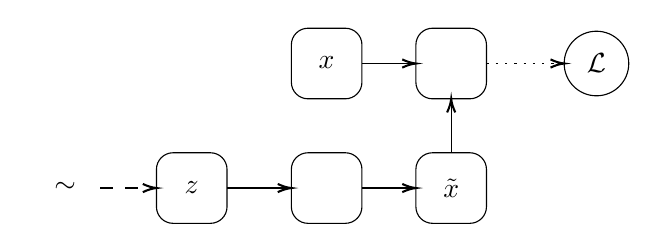
\begin{tikzpicture}[x=0.75pt,y=0.75pt,yscale=-1,xscale=1]
%uncomment if require: \path (0,159); %set diagram left start at 0, and has height of 159


% Text Node
\draw    (218,26) .. controls (218,21.58) and (221.58,18) .. (226,18) -- (244,18) .. controls (248.42,18) and (252,21.58) .. (252,26) -- (252,44) .. controls (252,48.42) and (248.42,52) .. (244,52) -- (226,52) .. controls (221.58,52) and (218,48.42) .. (218,44) -- cycle  ;
\draw (235,35) node   [align=left] {\begin{minipage}[lt]{20.400000000000002pt}\setlength\topsep{0pt}
\begin{center}
$\displaystyle \boldsymbol{x}$
\end{center}

\end{minipage}};
% Text Node
\draw    (153,86) .. controls (153,81.58) and (156.58,78) .. (161,78) -- (179,78) .. controls (183.42,78) and (187,81.58) .. (187,86) -- (187,104) .. controls (187,108.42) and (183.42,112) .. (179,112) -- (161,112) .. controls (156.58,112) and (153,108.42) .. (153,104) -- cycle  ;
\draw (170,95) node   [align=left] {\begin{minipage}[lt]{20.400000000000002pt}\setlength\topsep{0pt}
\begin{center}
$\displaystyle \boldsymbol{z}$
\end{center}

\end{minipage}};
% Text Node
\draw    (218,86) .. controls (218,81.58) and (221.58,78) .. (226,78) -- (244,78) .. controls (248.42,78) and (252,81.58) .. (252,86) -- (252,104) .. controls (252,108.42) and (248.42,112) .. (244,112) -- (226,112) .. controls (221.58,112) and (218,108.42) .. (218,104) -- cycle  ;
\draw (235,95) node   [align=left] {\begin{minipage}[lt]{20.400000000000002pt}\setlength\topsep{0pt}
\begin{center}
$\Generator$
\end{center}

\end{minipage}};
% Text Node
\draw    (278,26) .. controls (278,21.58) and (281.58,18) .. (286,18) -- (304,18) .. controls (308.42,18) and (312,21.58) .. (312,26) -- (312,44) .. controls (312,48.42) and (308.42,52) .. (304,52) -- (286,52) .. controls (281.58,52) and (278,48.42) .. (278,44) -- cycle  ;
\draw (295,35) node   [align=left] {\begin{minipage}[lt]{20.400000000000002pt}\setlength\topsep{0pt}
\begin{center}
$\Discriminator$
\end{center}

\end{minipage}};
% Text Node
\draw    (365, 35) circle [x radius= 15.56, y radius= 15.56]   ;
\draw (365,35) node   [align=left] {\begin{minipage}[lt]{13.735995849609345pt}\setlength\topsep{0pt}
\begin{center}
$\displaystyle \mathcal{L}$
\end{center}

\end{minipage}};
% Text Node
\draw (109,95) node   [align=left] {\begin{minipage}[lt]{20.400000000000002pt}\setlength\topsep{0pt}
\begin{center}
$\displaystyle \sim $
\end{center}

\end{minipage}};
% Text Node
\draw    (278,86) .. controls (278,81.58) and (281.58,78) .. (286,78) -- (304,78) .. controls (308.42,78) and (312,81.58) .. (312,86) -- (312,104) .. controls (312,108.42) and (308.42,112) .. (304,112) -- (286,112) .. controls (281.58,112) and (278,108.42) .. (278,104) -- cycle  ;
\draw (295,95) node   [align=left] {\begin{minipage}[lt]{20.400000000000002pt}\setlength\topsep{0pt}
\begin{center}
$\displaystyle \boldsymbol{\tilde{x}}$
\end{center}

\end{minipage}};
% Connection
\draw    (187,95) -- (216,95) ;
\draw [shift={(218,95)}, rotate = 180] [color={rgb, 255:red, 0; green, 0; blue, 0 }  ][line width=0.75]    (6.56,-1.97) .. controls (4.17,-0.84) and (1.99,-0.18) .. (0,0) .. controls (1.99,0.18) and (4.17,0.84) .. (6.56,1.97)   ;
% Connection
\draw    (252,35) -- (276,35) ;
\draw [shift={(278,35)}, rotate = 180] [color={rgb, 255:red, 0; green, 0; blue, 0 }  ][line width=0.75]    (6.56,-1.97) .. controls (4.17,-0.84) and (1.99,-0.18) .. (0,0) .. controls (1.99,0.18) and (4.17,0.84) .. (6.56,1.97)   ;
% Connection
\draw  [dash pattern={on 0.84pt off 2.51pt}]  (312,35) -- (347.44,35) ;
\draw [shift={(349.44,35)}, rotate = 180] [color={rgb, 255:red, 0; green, 0; blue, 0 }  ][line width=0.75]    (6.56,-1.97) .. controls (4.17,-0.84) and (1.99,-0.18) .. (0,0) .. controls (1.99,0.18) and (4.17,0.84) .. (6.56,1.97)   ;
% Connection
\draw  [dash pattern={on 4.5pt off 4.5pt}]  (126,95) -- (151,95) ;
\draw [shift={(153,95)}, rotate = 180] [color={rgb, 255:red, 0; green, 0; blue, 0 }  ][line width=0.75]    (6.56,-1.97) .. controls (4.17,-0.84) and (1.99,-0.18) .. (0,0) .. controls (1.99,0.18) and (4.17,0.84) .. (6.56,1.97)   ;
% Connection
\draw    (252,95) -- (276,95) ;
\draw [shift={(278,95)}, rotate = 180] [color={rgb, 255:red, 0; green, 0; blue, 0 }  ][line width=0.75]    (6.56,-1.97) .. controls (4.17,-0.84) and (1.99,-0.18) .. (0,0) .. controls (1.99,0.18) and (4.17,0.84) .. (6.56,1.97)   ;
% Connection
\draw    (295,78) -- (295,54) ;
\draw [shift={(295,52)}, rotate = 450] [color={rgb, 255:red, 0; green, 0; blue, 0 }  ][line width=0.75]    (6.56,-1.97) .. controls (4.17,-0.84) and (1.99,-0.18) .. (0,0) .. controls (1.99,0.18) and (4.17,0.84) .. (6.56,1.97)   ;

\end{tikzpicture}}
    \caption{A Generative Adversarial Network. Here, the tilde symbol over the vector yielded by the generator indicates that it does not come from the training set but it is generated. The discriminator $D$ must distinguish between generated and real samples (indicated without the tilde).}
    \label{fig:gan}
\end{figure*}
Notice that, in order to train the architecture of the model, the samples taken from the generator of a \gls{gan} must differentiable.